\documentclass[mathserif]{beamer}

\setbeamertemplate{frametitle}[default][center]%Centers the frame title.
\setbeamertemplate{navigation symbols}{}%Removes navigation symbols.
\setbeamertemplate{footline}{\raisebox{5pt}{\makebox[\paperwidth]{\hfill\makebox[10pt]{\scriptsize\insertframenumber}}}}
\setbeamertemplate{caption}[numbered]

\usepackage{amssymb,amsfonts,amsmath,latexsym,amsthm}
%\usepackage[usenames,dvipsnames]{color}
%\usepackage[]{graphicx}
%\usepackage[space]{grffile}
\usepackage{mathrsfs}   % fancy math font
% \usepackage[font=small,skip=0pt]{caption}
\usepackage[skip=0pt]{caption}
\usepackage{subcaption}
\usepackage{verbatim}
\usepackage{url}
\usepackage{bm}
\usepackage{dsfont}
\usepackage{extarrows}
\usepackage{multirow}
%\newcommand{\tth}   {\mbox{$\theta$}}
\newcommand{\thh}   {\mbox{$\theta$}}
\newcommand{\su}   {\mbox{$\sigma^2$}}
\newcommand{\so}   {\mbox{$\sigma_0^2$}}
\newcommand{\ko}   {\mbox{$\kappa_0$}}
\newcommand{\no}   {\mbox{$\nu_0$}}
\newcommand{\mo}   {\mbox{$\mu_0$}}
\newcommand{\ti}   {\mbox{$\tilde{x}$}}
\newcommand{\la}   {\mbox{$\lambda$}}
\newcommand{\bx}   {\mbox{$\bm{x}$}}
\newcommand{\bZ}   {\mbox{$\bm{Z}$}}
\newcommand{\bX}   {\mbox{$\bm{X}$}}
\newcommand{\bY}   {\mbox{$\bm{Y}$}}
\newcommand{\bA}   {\mbox{$\bm{A}$}}
\newcommand{\ba}   {\mbox{$\bm{a}$}}
\newcommand{\bb}   {\mbox{$\bm{b}$}}
\newcommand{\bt}   {\mbox{$\bm{t}$}}
\newcommand{\bz}   {\mbox{$\bm{z}$}}
\newcommand{\bw}   {\mbox{$\bm{w}$}}
\newcommand{\bbeta}   {\mbox{$\bm{\beta}$}}

\newcommand{\be}   {\mbox{$\bm{e}$}}
\newcommand{\bu}   {\mbox{$\bm{u}$}}
\newcommand{\bv}   {\mbox{$\bm{v}$}}
\newcommand{\sig}   {\mbox{$\Sigma$}}
\newcommand{\sigx}   {\mbox{$\Sigma_{XX}$}}
\newcommand{\sigxy}   {\mbox{$\Sigma_{XY}$}}
\newcommand{\tr}   {\mbox{$\text{tr}$}}
\newcommand{\ddet}   {\mbox{$\text{det}$}}
\newcommand\independent{\protect\mathpalette{\protect\independenT}{\perp}}
\def\independenT#1#2{\mathrel{\rlap{$#1#2$}\mkern2mu{#1#2}}}

\newcommand{\Expect}[1]{\ensuremath{\mathbf{E}\left[ #1 \right]}}
%\newcommand{\Var}[1]{\ensuremath{\mathrm{Var}\left[ #1 \right]}}
%\newcommand{\Cov}[1]{\ensuremath{\mathrm{Cov}\left[ #1 \right]}}
\newcommand{\MSE}{\ensuremath{\mathrm{MSE}}}
\newcommand{\RSS}{\ensuremath{\mathrm{RSS}}}
\newcommand{\Prob}[1]{\ensuremath{\mathrm{Pr}\left( #1 \right)}}
\newcommand{\ProbEst}[1]{\ensuremath{\widehat{\mathrm{Pr}}\left( #1 \right)}}
\DeclareMathOperator*{\argmin}{argmin} % thanks, wikipedia!
\DeclareMathOperator*{\argmax}{argmax} % thanks, wikipedia!
\DeclareMathOperator*{\sgn}{sgn} % thanks, wikipedia!

\newcommand{\lam}{\lambda}
\newcommand{\bmu}{\bm{\mu}}
%\newcommand{\bx}{\ensuremath{\mathbf{X}}}
\newcommand{\X}{\ensuremath{\mathbf{X}}}
\newcommand{\w}{\ensuremath{\mathbf{w}}}
\newcommand{\h}{\ensuremath{\mathbf{h}}}
\newcommand{\V}{\ensuremath{\mathbf{V}}}
%\newcommand{\tr}{\operatorname{tr}}

%\newcommand{\bx}{\ensuremath{\mathbf{X}}}
%\newcommand{\X}{\ensuremath{\mathbf{x}}}
%\newcommand{\w}{\ensuremath{\mathbf{w}}}
%\newcommand{\h}{\ensuremath{\mathbf{h}}}
%\newcommand{\V}{\ensuremath{\mathbf{v}}}
%\newcommand{\Cov}{\text{Cov}}
%\newcommand{\Var}{\text{Var}}

\DeclareMathOperator{\var}{Var}
\DeclareMathOperator{\cov}{Cov}
\newcommand{\Var}[1]{\ensuremath{\mathrm{Var}\left[ #1 \right]}}
\newcommand{\Cov}[1]{\ensuremath{\mathrm{Cov}\left[ #1 \right]}}


\newcommand{\indep}{\rotatebox{90}{\ensuremath{\models}}}
\newcommand{\notindep}{\not\hspace{-.05in}\indep}







\usepackage{float,bm}
\floatstyle{boxed}
\newfloat{code}{tp}{code}
\floatname{code}{Code Example}
%\newcommand{\tth}   {\mbox{$\theta$}}
\newcommand{\thh}   {\mbox{$\theta$}}
\newcommand{\su}   {\mbox{$\sigma^2$}}
\newcommand{\so}   {\mbox{$\sigma_0^2$}}
\newcommand{\ko}   {\mbox{$\kappa_0$}}
\newcommand{\no}   {\mbox{$\nu_0$}}
\newcommand{\mo}   {\mbox{$\mu_0$}}
\newcommand{\ti}   {\mbox{$\tilde{x}$}}
\newcommand{\la}   {\mbox{$\lambda$}}
\newcommand{\bx}   {\mbox{$\bm{x}$}}
\newcommand{\bZ}   {\mbox{$\bm{Z}$}}
\newcommand{\bX}   {\mbox{$\bm{X}$}}
\newcommand{\bY}   {\mbox{$\bm{Y}$}}
\newcommand{\bA}   {\mbox{$\bm{A}$}}
\newcommand{\ba}   {\mbox{$\bm{a}$}}
\newcommand{\bb}   {\mbox{$\bm{b}$}}
\newcommand{\bt}   {\mbox{$\bm{t}$}}
\newcommand{\bz}   {\mbox{$\bm{z}$}}
\newcommand{\bw}   {\mbox{$\bm{w}$}}
\newcommand{\bbeta}   {\mbox{$\bm{\beta}$}}

\newcommand{\be}   {\mbox{$\bm{e}$}}
\newcommand{\bu}   {\mbox{$\bm{u}$}}
\newcommand{\bv}   {\mbox{$\bm{v}$}}
\newcommand{\sig}   {\mbox{$\Sigma$}}
\newcommand{\sigx}   {\mbox{$\Sigma_{XX}$}}
\newcommand{\sigxy}   {\mbox{$\Sigma_{XY}$}}
\newcommand{\tr}   {\mbox{$\text{tr}$}}
\newcommand{\ddet}   {\mbox{$\text{det}$}}
\newcommand\independent{\protect\mathpalette{\protect\independenT}{\perp}}
\def\independenT#1#2{\mathrel{\rlap{$#1#2$}\mkern2mu{#1#2}}}

\newcommand{\Expect}[1]{\ensuremath{\mathbf{E}\left[ #1 \right]}}
%\newcommand{\Var}[1]{\ensuremath{\mathrm{Var}\left[ #1 \right]}}
%\newcommand{\Cov}[1]{\ensuremath{\mathrm{Cov}\left[ #1 \right]}}
\newcommand{\MSE}{\ensuremath{\mathrm{MSE}}}
\newcommand{\RSS}{\ensuremath{\mathrm{RSS}}}
\newcommand{\Prob}[1]{\ensuremath{\mathrm{Pr}\left( #1 \right)}}
\newcommand{\ProbEst}[1]{\ensuremath{\widehat{\mathrm{Pr}}\left( #1 \right)}}
\DeclareMathOperator*{\argmin}{argmin} % thanks, wikipedia!
\DeclareMathOperator*{\argmax}{argmax} % thanks, wikipedia!
\DeclareMathOperator*{\sgn}{sgn} % thanks, wikipedia!

\newcommand{\lam}{\lambda}
\newcommand{\bmu}{\bm{\mu}}
%\newcommand{\bx}{\ensuremath{\mathbf{X}}}
\newcommand{\X}{\ensuremath{\mathbf{X}}}
\newcommand{\w}{\ensuremath{\mathbf{w}}}
\newcommand{\h}{\ensuremath{\mathbf{h}}}
\newcommand{\V}{\ensuremath{\mathbf{V}}}
%\newcommand{\tr}{\operatorname{tr}}

%\newcommand{\bx}{\ensuremath{\mathbf{X}}}
%\newcommand{\X}{\ensuremath{\mathbf{x}}}
%\newcommand{\w}{\ensuremath{\mathbf{w}}}
%\newcommand{\h}{\ensuremath{\mathbf{h}}}
%\newcommand{\V}{\ensuremath{\mathbf{v}}}
%\newcommand{\Cov}{\text{Cov}}
%\newcommand{\Var}{\text{Var}}

\DeclareMathOperator{\var}{Var}
\DeclareMathOperator{\cov}{Cov}
\newcommand{\Var}[1]{\ensuremath{\mathrm{Var}\left[ #1 \right]}}
\newcommand{\Cov}[1]{\ensuremath{\mathrm{Cov}\left[ #1 \right]}}


\newcommand{\indep}{\rotatebox{90}{\ensuremath{\models}}}
\newcommand{\notindep}{\not\hspace{-.05in}\indep}






%\usepackage{fontspec}
%\setmainfont{Tahoma}

%\newcommand{\lam}{\lambda}
%\newcommand{\bmu}{\bm{\mu}}
%%\newcommand{\bx}{\ensuremath{\mathbf{X}}}
%\newcommand{\X}{\ensuremath{\mathbf{x}}}
%\newcommand{\w}{\ensuremath{\mathbf{w}}}
%\newcommand{\h}{\ensuremath{\mathbf{h}}}
%\newcommand{\V}{\ensuremath{\mathbf{v}}}
%\newcommand{\cov}{\text{Cov}}
%\newcommand{\var{\text{Var}}}

%\DeclareMathOperator{\var}{Var}
%\DeclareMathOperator{\cov}{Cov}

%\newcommand{\indep}{\rotatebox{90}{\ensuremath{\models}}}
%\newcommand{\notindep}{\not\hspace{-.05in}\indep}

\usepackage{graphicx} %The mode "LaTeX => PDF" allows the following formats: .jpg  .png  .pdf  .mps
\graphicspath{{./PresentationPictures/}} %Where the figures folder is located
\usepackage{listings}
\usepackage{media9}
\usepackage{movie15}
\addmediapath{./Movies/}

\newcommand{\beginbackup}{
   \newcounter{framenumbervorappendix}
   \setcounter{framenumbervorappendix}{\value{framenumber}}
}
\newcommand{\backupend}{
   \addtocounter{framenumbervorappendix}{-\value{framenumber}}
   \addtocounter{framenumber}{\value{framenumbervorappendix}} 
}


%\usepackage{algorithm2e}
\usepackage[ruled,lined]{algorithm2e}
\def\algorithmautorefname{Algorithm}
\SetKwIF{If}{ElseIf}{Else}{if}{then}{else if}{else}{endif}
%\usepackage{times}
%\usepackage[tbtags]{amsmath}
%\usepackage{amssymb}
\usepackage{amsfonts}
%\usepackage{slfortheorems}
\usepackage{epsfig}
\usepackage{graphicx}
%\usepackage[small]{caption}
%\usepackage[square]{natbib}
%\newcommand{\newblock}{}
%\bibpunct{(}{)}{;}{a}{}{,}
%\bibliographystyle{ims}
%\usepackage[letterpaper]{geometry}
%\usepackage{color}
%\setlength{\parindent}{0pt}

\usepackage{natbib}
\bibpunct{(}{)}{;}{a}{}{,}
%\usepackage{hyperref}

\DeclareMathOperator*{\Exp}{Exp}
\DeclareMathOperator*{\TExp}{TExp}
\DeclareMathOperator*{\Bernoulli}{Bernoulli}
\DeclareMathOperator*{\Beta}{Beta}
\DeclareMathOperator*{\Ga}{Gamma}
\DeclareMathOperator*{\TGamma}{TGamma}
\DeclareMathOperator*{\Poisson}{Poisson}
\DeclareMathOperator*{\Binomial}{Binomial}
\DeclareMathOperator*{\NormalGamma}{NormalGamma}
\DeclareMathOperator*{\InvGamma}{InvGamma}
\DeclareMathOperator*{\Cauchy}{Cauchy}
\DeclareMathOperator*{\Uniform}{Uniform}
\DeclareMathOperator*{\Gumbel}{Gumbel}
\DeclareMathOperator*{\Pareto}{Pareto}
\DeclareMathOperator*{\Mono}{Mono}
\DeclareMathOperator*{\Geometric}{Geometric}
\DeclareMathOperator*{\Wishart}{Wishart}

\newcommand{\R}{\mathbb{R}}
\newcommand{\Z}{\mathbb{Z}}
\newcommand{\E}{\mathbb{E}}
\renewcommand{\Pr}{\mathbb{P}}
\newcommand{\I}{\mathds{1}}
\newcommand{\V}{\mathbb{V}}

% Math operators
\DeclareMathOperator*{\diag}{diag}
\DeclareMathOperator*{\median}{median}
\DeclareMathOperator*{\Vol}{Vol}

% Miscellaneous commands
\newcommand{\iid}{\stackrel{\mathrm{iid}}{\sim}}
\newcommand{\matrixsmall}[1]{\bigl(\begin{smallmatrix}#1\end{smallmatrix} \bigr)}

\newcommand{\items}[1]{\begin{itemize} #1 \end{itemize}}

\newcommand{\todo}[1]{\emph{\textcolor{red}{(#1)}}}

\newcommand{\branch}[4]{
\left\{
	\begin{array}{ll}
		#1  & \mbox{if } #2 \\
		#3 & \mbox{if } #4
	\end{array}
\right.
}

% approximately proportional to
\def\app#1#2{%
  \mathrel{%
    \setbox0=\hbox{$#1\sim$}%
    \setbox2=\hbox{%
      \rlap{\hbox{$#1\propto$}}%
      \lower1.3\ht0\box0%
    }%
    \raise0.25\ht2\box2%
  }%
}
\def\approxprop{\mathpalette\app\relax}

\newcommand{\btheta}{{\bm\theta}}
\newcommand{\bbtheta}{{\pmb{\bm\theta}}}

%\usepackage{zref-savepos}
%
%\newcounter{restofframe}
%\newsavebox{\restofframebox}
%\newlength{\mylowermargin}
%\setlength{\mylowermargin}{2pt}
%
%\newenvironment{restofframe}{%
%    \par%\centering
%    \stepcounter{restofframe}%
%    \zsavepos{restofframe-\arabic{restofframe}-begin}%
%    \begin{lrbox}{\restofframebox}%
%}{%
%    \end{lrbox}%
%    \setkeys{Gin}{keepaspectratio}%
%    \raisebox{\dimexpr-\height+\ht\strutbox\relax}[0pt][0pt]{%
%    \resizebox*{!}{\dimexpr\zposy{restofframe-\arabic{restofframe}-begin}sp-\zposy{restofframe-\arabic{restofframe}-end}sp-\mylowermargin\relax}%
%        {\usebox{\restofframebox}}%
%    }%
%    \vskip0pt plus 1filll\relax
%    \mbox{\zsavepos{restofframe-\arabic{restofframe}-end}}%
%    \par
%}


\usepackage{tikz}
\usetikzlibrary{arrows}

%\usepackage[usenames,dvipsnames]{xcolor}
\usepackage{tkz-berge}
\usetikzlibrary{fit,shapes}

\usepackage{calc}
%%
%% The tikz package is used for doing the actual drawing.
%\usepackage{tikz}
%%
%% In order to be able to put arrowheads in the middle of directed edges, we need an extra library.
\usetikzlibrary{decorations.markings}
%%
%% The next line says how the "vertex" style of nodes should look: drawn as small circles.
\tikzstyle{vertex}=[circle, draw, inner sep=0pt, minimum size=6pt]
%%
%% Next, we make a \vertex command as a shorthand in place of \node[vertex} to get that style.
\newcommand{\vertex}{\node[vertex]}
%%
%% Finally, we declare a "counter", which is what LaTeX calls an integer variable, for use in
%% the calculations of angles for evenly spacing vertices in circular arrangements.
\newcounter{Angle}

\newtheoremstyle{example}
{\topsep} % space above
{\topsep} % space below
{} % body font
{} % indent
{\bf} % head font
{:} % punctuation between head and body
{0.5em} % space after head
{} % manually specify head
%{\thmname{#1}\thmnumber{ #2}\thmnote{:#3}} % manually specify head

\theoremstyle{example}
\newtheorem{ex}{Example}[section]

\newtheoremstyle{definition}
{\topsep} % space above
{\topsep} % space below
{} % body font
{} % indent
{\sc} % head font
{:} % punctuation between head and body
{0.5em} % space after head
{} % manually specify head
%{\thmname{#1}\thmnumber{ #2}\thmnote{:#3}} % manually specify head

\theoremstyle{definition}
\newtheorem{defn}{Definition}[section]

\theoremstyle{rem}
\newtheorem{rem}{Remark}[section]

\newtheoremstyle{theorem}
{\topsep} % space above
{\topsep} % space below
{} % body font
{} % indent
{\sc} % head font
{:} % punctuation between head and body
{0.5em} % space after head
{} % manually specify head
%{\thmname{#1}\thmnumber{ #2}\thmnote{:#3}} % manually specify head

\theoremstyle{theorm}
\newtheorem{thm}{Theorem}[section]



%%%to add in new counter for slides in beamer

%\setbeamertemplate{footline}{
%  \leavevmode%
%  \hbox{%
%  \begin{beamercolorbox}[wd=.333333\paperwidth,ht=2.25ex,dp=1ex,center]{author in head/foot}%
%    \usebeamerfont{author in head/foot}\insertshortauthor~~(\insertshortinstitute)
%  \end{beamercolorbox}%
%  \begin{beamercolorbox}[wd=.333333\paperwidth,ht=2.25ex,dp=1ex,center]{title in head/foot}%
%    \usebeamerfont{title in head/foot}\insertshorttitle
%  \end{beamercolorbox}%
%  \begin{beamercolorbox}[wd=.333333\paperwidth,ht=2.25ex,dp=1ex,right]{date in head/foot}%
%    \usebeamerfont{date in head/foot}\insertshortdate{}\hspace*{2em}
%    \insertframenumber{} \hspace*{2ex} % hier hat's sich ge�ndert
%  \end{beamercolorbox}}%
%  \vskip0pt%
%}



%%%%%

\newcommand*\oldmacro{}
\let\oldmacro\insertshortauthor
\renewcommand*\insertshortauthor{
  \leftskip=.3cm
\insertframenumber\,/\,\inserttotalframenumber\hfill\oldmacro}




%\excludecomment{notbeamer}
%\includecomment{beamer}



\title{Intro to Monte Carlo, Part I}
\author{Rebecca C. Steorts \\ Bayesian Methods and Modern Statistics: STA 360/601}
\date{Module 5}

\begin{document}

\maketitle


\frame{
\frametitle{Studying for an Exam}
\begin{enumerate}
\item The PhD notes
\item Homework
\item Lab (it's duplicated for a reason)
\item Class modules
\item Questions you ask me
\end{enumerate}
}

\frame{
\frametitle{How I write the exam}
\begin{enumerate}
\item I sit down and I go through the slides
\item I think about what we talked about in class
\item I look at what I assigned for your for reading in the notes, homework,
Hoff, and labs.
\item I think about the big concepts and I write problems to test your knowledge of this. 
\end{enumerate}
}

\frame{
\frametitle{Where many of your went wrong}
\begin{enumerate}
\item You derived the Normal-Normal (you wasted time). 
\item You froze on the exam -- it happens.
\item You didn't use your time wisely. 
\item You wrote nothing down for some problems. 
\item Advice: write down things that make sense. We know when you're writing things 
down that are wrong. (Like when I make a typo in class).  
\end{enumerate}
}

\frame{
\frametitle{How to turn your semester around}
\begin{enumerate}
\item Have perfect homework grades
\item Start preparing for midterm 2 now. (It's on March 10th). 
\item You midterm grades were a worst case scenario.
\item There will be a curve and most of your grades will keep going up. (READ THIS AGAIN). 
\item Keep working hard. (And yes, I know you're all working very hard).
\item Undergrads: stay after class for a few minutes. I want to talk to you apart from the grad students. 
\end{enumerate}
}

\frame{
\frametitle{Where we are in Hoff, notes, class, labs}

\begin{enumerate}
\item Homework 4: posted and due March 2, 11:55 PM. 
\item Lab next week: importance and rejection sampling
\item Lab before midterm 2: Gibbs sampling
\item Class: importance sampling, rejection, and Gibbs sampling. 
\end{enumerate}




}






\frame{
Goal: approximate
$$\textcolor{red}{\int_X h(x) f(x)\; dx}$$ that is intractable, where $f(x)$ is a probability density. 

\vskip 2em
What's the problem? Typically $h(x)$ is messy! 

\vskip 2em
Why not use numerical integration techniques? 

\vskip 2em
In dimension $d=3$ or higher, Monte carlo really improves upon numerical integration. 
}



\frame{
\frametitle{Numerical integration}


\begin{itemize}
%\item The most serious problem is the so-called ``curse of dimensionality.''  

\item Suppose we have a $d$-dimensional integral.  
\item Numerical integration typically entails evaluating the integrand over some grid of points.  
\item However, if $d$ is even moderately large, then any reasonably fine grid will contain an impractically large number of points.  
\end{itemize}
}

\frame{
\frametitle{Numerical integration}
\begin{itemize}
\item Let $d=6$. Then a grid with just ten points in each dimension will consist of $10^6$ points.  
\item If $d=50$, then even an absurdly coarse grid with just \emph{two} points in each dimension will consist of $2^{50}$ points (note that $2^{50}>10^{15}$).
\end{itemize}
%\item There can still be problems even when the dimensionality is small.  There are packages in \texttt{R} called \textbf{area} and \textbf{integrate}, however, area cannot deal with infinite bounds in the integral, and even though integrate can handle infinite bounds, it is fragile and often produces output that's not trustworthy (Robert and Casella, 2010).

\emph{What's happening here?}

}

\frame{
\frametitle{Numerical integration error rates (big Ohh concepts)}
%Suppose X is O(n). This means that $X \stackrel{\rightarrow}{p} 

If $d=1$ and we assume crude numerical integration based on a grid size $n$, then we typically get an error of order $n^{-1}.$

\vskip 1 em

For most dimensions $d,$ estimates based on numerical integrations required $m^d$ evaluations to achieve an error of $m^{-1}.$

\vskip 1 em

Said differently, with $n$ evaluations, you get an error of order $n^{-1/d}.$

\vskip 1 em

But, the Monte Carlo estimate retains an error rate of $n^{-1/2}.$\\
(The constant in this error rate may be quite large).

}

\frame{
\frametitle{Classical Monte Carlo Integration}

The generic problem here is to evaluate 
$$\textcolor{red}{E_f[h(x)] = \int_X h(x) f(x) \; dx.}$$
\vskip 1em
The classical way to solve this is generate a sample $(X_1,\ldots,X_n)$ from $f.$ 
\vskip 1 em
Now propose as an approximation the empirical average:
$$\bar{h}_n = \frac{1}{n}\sum_{j=n}^n h(x_j).$$ 
\vskip 1 em
Why?  $\bar{h}_n$ converges a.s.\ (i.e.\ for almost every generated sequence) to $E_f[h(X)]$ by the Strong Law of Large Numbers. 

}

\frame{

Also, under certain assumptions\footnote{see Casella and Robert, page 65, for details}, the asymptotic variance can be approximated and then can be estimated from the sample $(X_1,\ldots,X_n)$ by 
$$v_n = 1/n \sum_{j=1}^n [h(x_j) - \bar{h}_n]^2.$$ Finally, by the CLT (for large $n$), 
$$\frac{\bar{h}_n - E_f[h(X)]}{\sqrt v_n} \;\stackrel{\text{approx.}}{\sim}\; N(0,1).$$

(Technically, it converges in distribution). 


}

\frame{
\frametitle{Importance Sampling}

%Importance sampling involves generating random variables from a different distribution and then reweighing the output. It's name is given since the new distribution is chosen to give greater mass to regions where $h$ is large (the important part of the space).

Recall that we have a difficult, problem child of a function $h(x)!$

\begin{itemize}
\item Generate samples from a distribution $g(x).$
\item We then ``re-weight" the output.
\end{itemize}

\vskip 1em
Note: $g$ is chosen to give greater mass to regions where $h$ is large (the important part of the space).
\vskip 1em
This is called \emph{importance sampling.}


}


\frame{
\frametitle{Importance Sampling}

Let $g$ be an arbitrary density function and then we can write 
\begin{align}
\label{is}
I = E_f[h(x)] = \int_X h(x) \frac{f(x)}{g(x)} {g(x)}\; dx = 
E_g\left[\frac{h(x)f(x)}{g(x)}\right].
\end{align}
%This importance sampling fundamental identity justifies the use of the estimator
This is estimated by
\begin{align}
\label{is2}
\hat{I} = 
\frac{1}{n} \sum_{j=1}^n \frac{f(X_j)}{g(X_j)}
h(X_j) \longrightarrow  
E_f[h(X)]
\end{align}
based on a sample generated from $g$ (not $f$). Since (\ref{is}) can be written as an expectation under $g$, (\ref{is2}) converges to (\ref{is}) for the same reason the Monte carlo estimator $\bar{h}_n$ converges.



}

\frame{
\frametitle{The Variance}

\begin{align}
Var(\hat{I}) &= \dfrac{1}{n^2}\sum_i Var\left(\dfrac{h(X_i) f(X_i)}{g(X_i)}\right)\\
&=\dfrac{1}{n}Var\left(\dfrac{h(X_i) f(X_i)}{g(X_i)}\right)  \implies \\
\widehat{Var}(\hat{I}) &= 
\dfrac{1}{n}\widehat{Var}\left(\dfrac{h(X_i) f(X_i)}{g(X_i)}\right).
\end{align}


}

\frame{
\frametitle{Simple Example}

Suppose we want to estimate $P(X>5),$ where $X \sim N(0,1).$ \\

\vskip 1 em
\textbf{Naive method}: 
\begin{itemize}
\item Generate $X_1 \ldots X_n \stackrel{iid}{\sim} N(0,1)$
\item Take the proportion $\hat{p} = \bar{X} > 5$ as your estimate
\end{itemize}
%Generate n iid standard normals and use the proportion $\hat{p}$ that are larger than 5.
\textbf{Importance sampling method}:
\begin{itemize} 
\item Sample from a distribution that gives high probability to the ``important region" (the set $(5, \infty)$).
\item Do re-weighting.
\end{itemize}
}



\frame{
\frametitle{Importance Sampling Solution}
 Let $f = \phi_o$ and $g = \phi_{\theta}$ be the densities of the $N(0,1)$ and $N(\theta,1)$ distributions ($\theta$ taken around 5 will work). Then
\begin{align} p &= \int I(u > 5) \phi_o(u)\; du \\
 &= 
\int \left[ I(u > 5) \frac{\phi_o(u)}{\phi_{\theta}(u)}
\right]
\phi_{\theta}(u)
\; du.
\end{align}
In other words, if 
$$ h(u) = I(u>5)\frac{\phi_o(u)}{\phi_{\theta}(u)}$$
then $p = E_{\phi_{\theta}}[h(X)].$
\vskip 1em
If
$X_1, \ldots, X_n \sim N(\theta, 1),$ then an unbiased estimate is 
$\hat{p} = \frac{1}{n} \sum_i  h(X_i).$


}

\begin{frame}[fragile]
\frametitle{Simple Example Code}
\begin{verbatim}

1 - pnorm(5)                  # gives 2.866516e-07
## Naive method
set.seed(1)
mySample <- 100000
x <- rnorm(n=mySample)
pHat <- sum(x>5)/length(x)
sdPHat <- sqrt(pHat*(1-pHat)/length(x)) # gives 0

## IS method

set.seed(1)
y <- rnorm(n=mySample, mean=5)
h <- dnorm(y, mean=0)/dnorm(y, mean=5) * I(y>5)
mean(h)                       # gives 2.865596e-07
sd(h)/sqrt(length(h))         # gives 2.157211e-09
\end{verbatim}
\textcolor{blue}{Notice the difference between the naive method and IS method!}
\end{frame}

\frame{
\frametitle{Harder example}

Let $f(x)$ be the pdf of a $N(0,1)$. Assume we want to compute $$a = \int_{-1}^{1}{f(x)dx} =  \int_{-1}^{1}{N(0,1)dx}$$ 

\vskip 1em

Let $g(X)$ be an arbitrary pdf, $$a(x) = \int_{-1}^{1}{\frac{f(x)}{g(x)} g(x)\;dx}.$$

\vskip 1em

We want to be able to draw $g(x) \sim Y$ easily. But how should we go about choosing $g(x)?$

}


\frame{
\frametitle{Harder example}

\begin{itemize}
\item Note that if $g \sim Y,$ then 
$a = E[I_{[-1,1]}(Y)\frac{f(Y)}{g(Y)}]$.  
%\item The variance of $I_{[-1,1]}(Y)\dfrac{f(Y)}{g(Y)}$ is minimized picking $g \propto I_{[-1,1]}(x)f(x)$. Nevertheless simulating from this $g$ is usually expensive.
\item Some $g$'s which are easy to simulate from are the pdf's of:
\begin{itemize}
\item  the $\text{Uniform}(-1,1)$, 
\item the Normal$(0,1),$ 
\item and a Cauchy with location parameter $0$ (Student t with 1 degree of freedom). 
\end{itemize}
\item Below, there is code of how to get a sample from $$I_{[-1,1]}(Y)\dfrac{f(Y)}{g(Y)}$$ for the three choices of $g.$ 
\end{itemize}

}


\begin{frame}[fragile]
\frametitle{Harder example}

\begin{verbatim}
uniformIS <- function(sampleSize=10) {
  sapply(runif(sampleSize,-1,1), 
    function(xx) dnorm(xx,0,1)/dunif(xx,-1,1)) }

cauchyIS <- function(sampleSize=10) {
  sapply(rt(sampleSize,1), 
    function(xx) 
    (xx <= 1)*(xx >= -1)*dnorm(xx,0,1)/dt(xx,2)) }

gaussianIS <- function(sampleSize=10) {
  sapply(rnorm(sampleSize,0,1),
    function(xx) (xx <= 1)*(xx >= -1)) }
\end{verbatim}

\end{frame}

\frame{


\begin{figure}
	\centering
	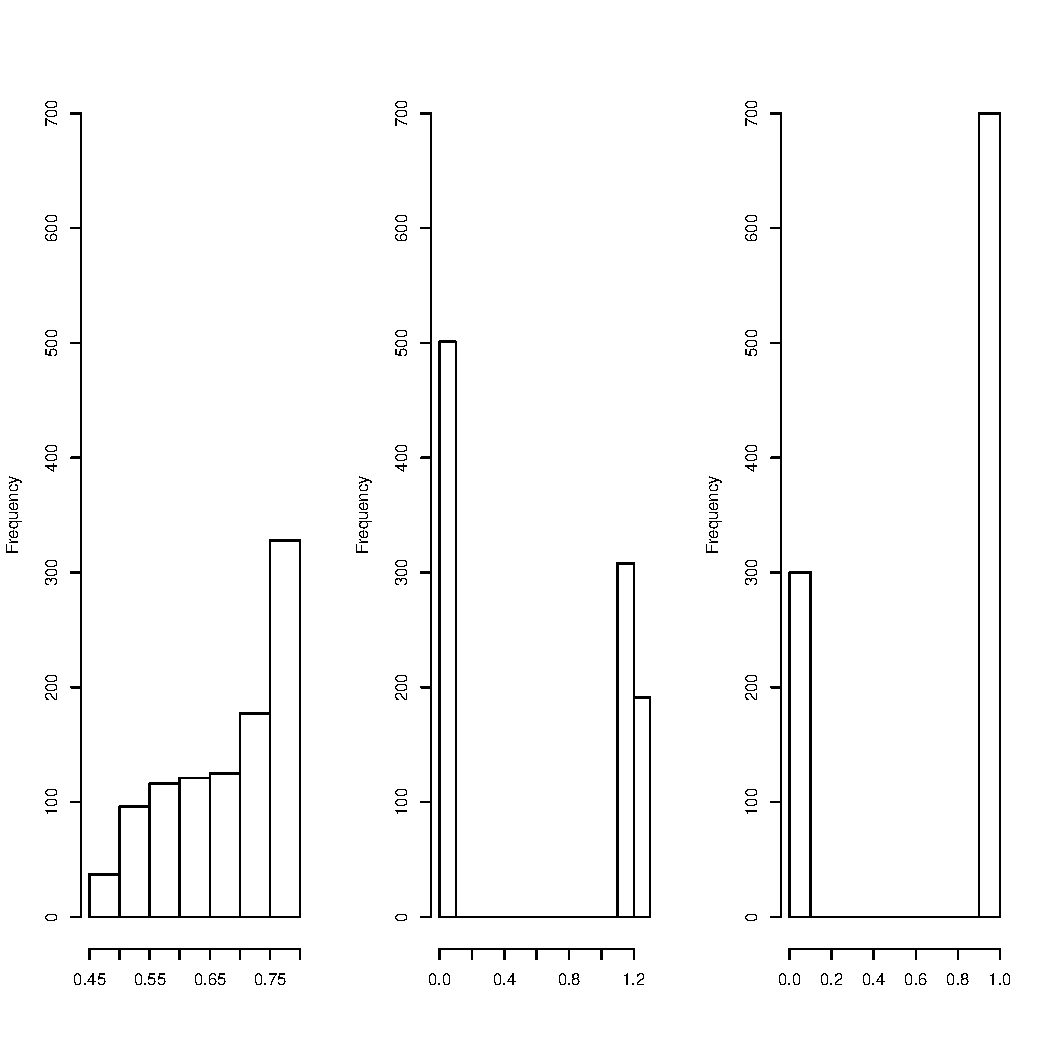
\includegraphics[scale=0.45]{importance_sampling2}
	\caption{Histograms for samples from $I_{[-1,1]}(Y)\frac{f(Y)}{g(Y)}$ when $g$ is, respectivelly, a uniform, a Cauchy and a Normal pdf.}
	\label{ex2.IS.gaussian}
\end{figure}


}

\frame{
\frametitle{Importance Sampling with unknown normalizing constant}

Often we have sample from $\mu$, but know $\textcolor{blue}{\pi(x)}$ except for a multiplicative $\mu(x)$ constant. Typical example is Bayesian situation:

\begin{itemize}
\item $\textcolor{blue}{\pi(x)}= \nu_Y =$ posterior of $\theta \mid Y$ when prior density is $\nu.$
\item $\mu(x) = \lambda_Y$ = posterior of $\theta \mid Y$ when prior density is  $\lambda.$\footnote{I'm motivating this in a Bayesian context. The way Hoff writes this  is equivalent.}
\end{itemize}

\vskip 1em 
Consider $$\dfrac{\textcolor{blue}{\pi(x)}}{\mu(x)} = \dfrac{c_{\nu} L(\theta) \nu(\theta)}
{c_{\lambda} L(\theta) \lambda(\theta)} = c \dfrac{\nu(\theta)} {\lambda(\theta)} =c\; \ell(x),$$

where $\ell(x)$ is known and $c$ is unknown.

\vskip 1em 

This implies that $$\textcolor{blue}{\pi(x)} = c\; \ell(x) \mu(x).$$





}

\frame{
Then if we're estimating $h(x)$, we find 
\begin{align}
\int h(x) \pi(x) \;dx
&= 
\int h(x)\; c \; \ell(x) \mu(x) \; d(x)\\
&= \frac{\int h(x) \;c \; \ell(x) \mu(x) \; d(x)}
{\int  \pi(x) \; d(x)}\\
&= \frac{\int h(x) \;c \; \ell(x) \mu(x) \; d(x)}
{\int  c \; \ell(x) \mu(x) \; d(x)}\\
&= \frac{\int h(x) \; \ell(x) \mu(x) \; d(x)}
{\int   \ell(x) \mu(x) \; d(x)}.
\end{align}

Generate $X_1,\ldots,X_n \sim \mu$ and estimate via
$$\frac{\sum_i h(X_i) \; \ell(X_i)}{\sum_i\ell(X_i)} = 
\sum_i h(X_i) \left(
\frac{\ell(X_i)}
{
\sum_j \ell(X_j)
}
\right)
=
\sum_i w_i h(X_i)
$$
where 
$w_i = \dfrac{\ell(X_i)}
{
\sum_j \ell(X_j)
}
=\dfrac{\nu(\theta_i)/\lambda(\theta_i)}
{\sum_j \nu(\theta_j)/\lambda(\theta_j)}.
$

}

\frame{

Why the choice above for $\ell(X)?$ Just taking a ratio of priors. The motivation is the following for example: 

\begin{itemize}
\item Suppose our application is to Bayesian statistics where $\theta_1,\ldots,\theta_n \sim
\lambda_Y.$
%\item Think about the posterior corresponding here is an essay to deal with conjugate prior $\lambda.$
\item Think of $\pi = \nu$ as a complicated prior.
\item Think of  $\mu = \lambda$ as a conjugate prior.
\item Then the weights are $w_i = \dfrac{\nu(\theta_i)/\lambda(\theta_i)}
{\sum_j \nu(\theta_j)/\lambda(\theta_j)}.
$

\end{itemize}
}

\frame{
\begin{enumerate}
\item If $\mu$ and $\pi$ i.e. $\nu$ and $\lambda$ differ greatly most of the weight will be taken up by a few observations resulting in an unstable estimate. 

\item We can get an estimate of the variance of $$\sum_i \dfrac{h(X_i) \; \ell(X_i)}{\ell(X_i)}$$ but we need to use theorems from advance probability theory (The Cramer-Wold device and the Multivariate Delta Method). These details are beyond the scope of the class.

\item In Bayesian statistics, the cancellation of a potentially very complicated likelihood can lead to a great simplification. 

\item The original purpose of importance sampling was to sample more heavily from regions that are important. So, we may do importance sampling using a density $\mu$ because it's more convenient than using a density $\pi.$ (These could also be measures if the densities don't exist for those taking measure theory).
\end{enumerate}



}

%\frame{
%\frametitle{Animal-tracking GPS measurements, with extreme outliers. (Urbano et al., 2014)}
%
%
%
%\begin{figure}
%  \begin{center}
%    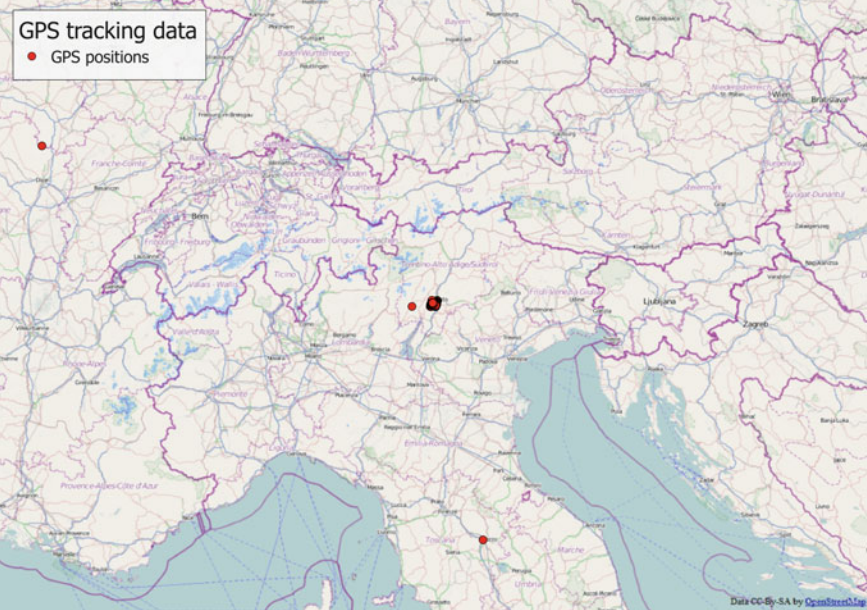
\includegraphics[width=0.8\textwidth]{urbano-GPS-outliers.png}
%    % Source: http://ase-research.org/basille/pubs/Urbano_2014b.pdf
%    %   Urbano, Ferdinando, Mathieu Basille, and Francesca Cagnacci. "Data Quality: Detection and Management of Outliers." Spatial Database for GPS Wildlife Tracking Data. Springer International Publishing, 2014. 115-137.
%    % License: ???
%    % Date accessed: 1/31/2014
%  \end{center}
%  \caption{Animal-tracking GPS measurements, with extreme outliers. (Urbano et al., 2014)}
%  \label{figure:urbano-GPS-outliers}
%\end{figure}
%
%}
%
%
%\frame{
%
%\begin{itemize}
%\item Animals are tagged with GPS devices in order to track their movements and study their behavior. The latitude/longitude measurements made by GPS devices are usually accurate, but it is not uncommon to get extreme outliers. 
%\item  Figure \ref{figure:urbano-GPS-outliers}  shows GPS measurements in northern Italy, with three extreme outliers visible.\footnote{One of which is way down toward central Italy, and another of which is clear across Switzerland and well into France!}
%\item The Normal (Gaussian) model is not robust to outliers, and if used naively in a situation like this, would give completely bogus results. (Homework part one: verify this). 
%\end{itemize}
%
%}
%
%
%%
%\frame{
%\frametitle{Animal-tracking GPS measurements, with extreme outliers. (Urbano et al., 2014)}
%
%How can we deal with such outliers? 
%
%To illustrate, consider the following 8 latitude/longitude points, one of which is an outlier:
%
%\begin{center}
%\begin{tabular}{ll}
%Latitude & Longitude \\
%\hline
%36.077916 N & 79.009266 W \\
%36.078032 N & 79.009180 W \\
%36.078129 N & 79.009094 W \\
%36.078048 N & 79.008891 W \\
%36.077942 N & 79.008962 W \\
%36.089612 N & 79.035760 W \\
%36.077789 N & 79.008917 W \\
%36.077563 N & 79.009281 W \\
%\end{tabular}
%\end{center}
%
%}
%%
%\frame{
%\frametitle{Animal-tracking GPS measurements, with extreme outliers. (Urbano et al., 2014)}
%
%To keep things simple, let's just consider the latitudes, and let's assume these points are collected in a short enough amount of time that the animal has not moved very far.Let's model the latitudes as
%$$X_1,\ldots,X_n\iid \Cauchy(\theta,s).$$
%Recall that the Cauchy distribution with location $\theta$ and scale $s$ has p.d.f.
%$$\Cauchy(x\mid \theta, s) = \frac{1}{\pi s \Big(1 + \big(\frac{x-\theta}{s}\big)^2\Big)}.$$
%Unfortunately, there is not a nice conjugate prior for $\theta$. Let's put a Cauchy prior on $\theta$:
%$$\btheta\sim \Cauchy(\theta_0,s_0).$$
%
%Suppose \begin{itemize}
%    \item scale of measurement errors: $s = 0.0002$ degrees (known, say, from calibration testing or instrument specifications)
%    \item center of prior on location: $\theta_0 = 36.07$ degrees (estimated, say, from many previous measurements for this animal)
%    \item scale of prior on location: $s_0 = 0.02$ degrees (estimated, say, from many previous measurements for this animal)
%\end{itemize}
%
%}

\frame{
\frametitle{Rejection Sampling}

Rejection sampling is a method for drawing random samples from a distribution whose p.d.f.\ can be evaluated up to a constant of proportionality. 

%\vskip 1 em
%Compared with the inverse c.d.f.\ method, rejection sampling has the advantage of working on complicated multivariate distributions.

\vskip 1 em

Difficulties? You must design a good proposal distribution (which can be difficult, especially in high-dimensional settings).

}

\frame{
\frametitle{Uniform Sampler}

Goal: Generate samples from Uniform(A), where A is complicated. 

\vskip 1 em

Example: $X \sim $ Uniform(Mandelbrot).

\vskip 1 em

How? Consider $I_X(A).$


\begin{figure}
  \begin{center}
    
\includegraphics[width=0.45\textwidth]{madel}
%    \hspace{0.05\textwidth}
%    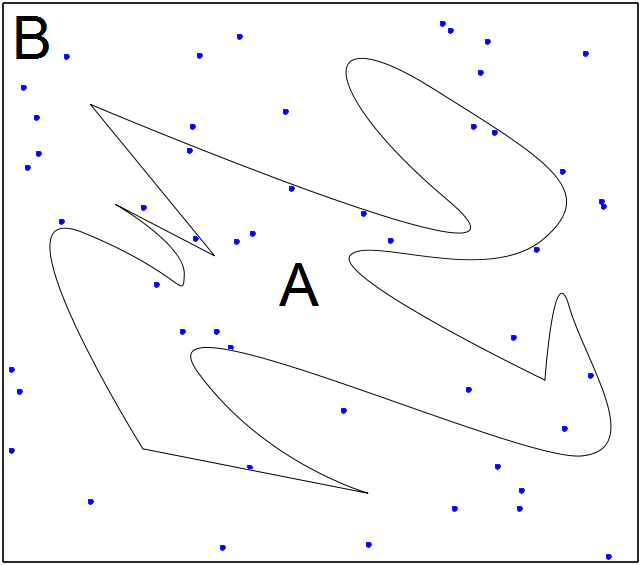
\includegraphics[width=0.45\textwidth]{code/reject-w-samples.png}
%    % Source: Original work by Jeffrey W. Miller
%    % Date: 2/1/2014
  \end{center}
  \caption{A complicated function $A,$ called the Mandelbrot!}
%  \label{figure:reject}
\end{figure}


}

\frame{
\frametitle{Proposition}
\begin{itemize}
\item Suppose $A \subset B.$ 
\item Let $Y_1,Y_2,\ldots \sim$ Uniform(B) iid and
\item  $X = Y_k$
where $k= \min \{k: Y_k \in A\},$ 
\end{itemize}
Then it follows that
$$X \sim \text{Uniform}(A).$$

Proof: Exercise. Hint: Try the discrete case first and use a geometric series. 



}

\frame{

\begin{figure}
  \begin{center}
    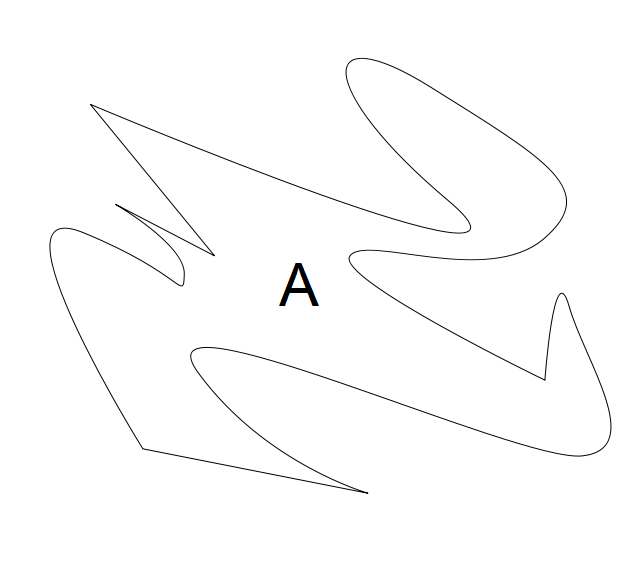
\includegraphics[width=0.45\textwidth]{code/reject-wo-samples.png}
    \hspace{0.05\textwidth}
    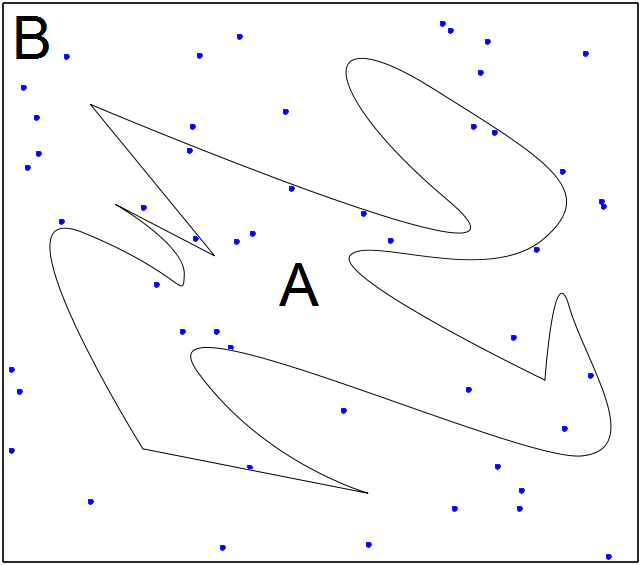
\includegraphics[width=0.45\textwidth]{code/reject-w-samples.png}
    % Source: Original work by Jeffrey W. Miller
    % Date: 2/1/2014
  \end{center}
  \caption{(Left) How to draw uniform samples from region $A$? (Right) Draw uniform samples from $B$ and keep only those that are in $A$.}
  \label{figure:reject}
\end{figure}

}

%\frame{
%\frametitle{Simple Rejection Sampling Formally Written}
%\begin{itemize}
%\item Let $\pi$ be a density. Suppose $$\pi(x) = c \;\ell(x),$$ where $\ell$ is known, $c$ is  unknown. 
%\item We are interested in case where \textcolor{blue}{$\pi$ is complicated}.
%\item Goal: Generate $X \sim \pi.$
%\end{itemize}
%
%{Simple rejection sampling}
%\begin{itemize}
%\item We're going to place a ``uniform box" over $\pi(x)$.
%\item Assume $\ell(x)$ is bounded and is zero outside of $[0, 1].$
%\item Suppose also $\ell(x)$ is constant on the intervals $$((j - 1)/k, j/k), j = 1,\ldots, k.$$ 
%\item Let $M$ be such that $M \geq \ell(x)$ for all $x.$
%\end{itemize}
%
%
%}

%\frame{
%\frametitle{Simple Rejection Sampling Algorithm}
%For very the very simple case, consider the following procedure.
%\begin{enumerate}
%\item Generate a point $(U_1, U_2)$ uniformly at random from the rectangle of
%height $M$ sitting on top of the interval $[0, 1].$
%\item If the point is below the graph of the function $\ell$, retain $U_1.$ Else, reject the point and go back to (1).
%\end{enumerate}
%
%\vskip 1 em
%
%Remark: Using the Probability Integral Transformation in reverse. If $X \sim F^{-1}(U),$ then $X \sim F$ where $U \sim \text{Uniform}(0,1).$
%
%\vskip 1 em
%
%%Remark: Think about what this is doing, we're generating many draws that are wasting time. Think about the restriction on $[0,1]$ and if this makes sense. 
%
%}

\frame{
\frametitle{General Rejection Sampling Algorithm}
%Let $\pi$ be a density. Suppose $$\pi(x) = c \;\ell(x),$$ where $\ell$ is known, $c$ is  unknown. 
Goal: Sample from a \textcolor{red}{complicated pdf $f(x).$}
\vskip 1 em
Suppose that $$\textcolor{red}{f(x)} = \tilde{f}(x)/\alpha, \alpha>0$$.

Algorithm: 


%Suppose the density $g$ is such that for some known constant $M,$ 
%$$Mg(x) \geq \ell(x)$$ for all $x.$
%Procedure:
\begin{enumerate}
\item Choose a \textcolor{blue}{proposal distribution $q$} such that $c>0$ with 
$$c \textcolor{blue}{q(x)} \geq \tilde{f}(x).$$
\item Sample $X \sim \textcolor{blue}{q}$, sample $Y \sim \text{Unif}(0, c\; \textcolor{blue}{q(X)})$ (given X)
\item If $Y \leq \tilde{f}(X), Z=X,$ we reject and return to step (2). 
%Generate $X \sim g,$ and calculate $r(X) = \dfrac{\ell(X)}{M\; g(X)}.$
%\item Flip a coin with probability of success $r(X).$ If we have a success,
%retain X. Else return to (1).
\end{enumerate}
Output: $Z \sim f$\\
Proof: Exercise.
}
%\frame{
%\frametitle{General Rejection Sampling Algorithm}
%To show that an accepted point has distribution $\pi$, let \textcolor{blue}{$I$ be the indicator that
%the point is accepted.} Then
%\begin{align}
%P(I=1) &= \int P(I=1 \mid X=x) g(x) \; dx\\
%& = \int \frac{\ell(x)}{M\; g(x)} g(x)\; dx \\
%&= \int \frac{\pi(x)/c}{M\; g(x)} g(x)\; dx \\
%&= 
%\frac{1}{c\; M} \int \pi(x) \; dx \\
%&= 
%\frac{1}{c\; M}.
%\end{align}
%
%Thus, if $g_\ell$ is the conditional distribution of $X$ given $I,$ we have
%\begin{align}
%g_I(x | I=1) &= P(x, I = 1)/ P(I=1)\\
%&=
%g(x) \frac{\pi(x)/c}{M\; g(x)} / P(I=1) = \pi(x).
%\end{align}
%}

\frame{


\begin{figure}
  \begin{center}
    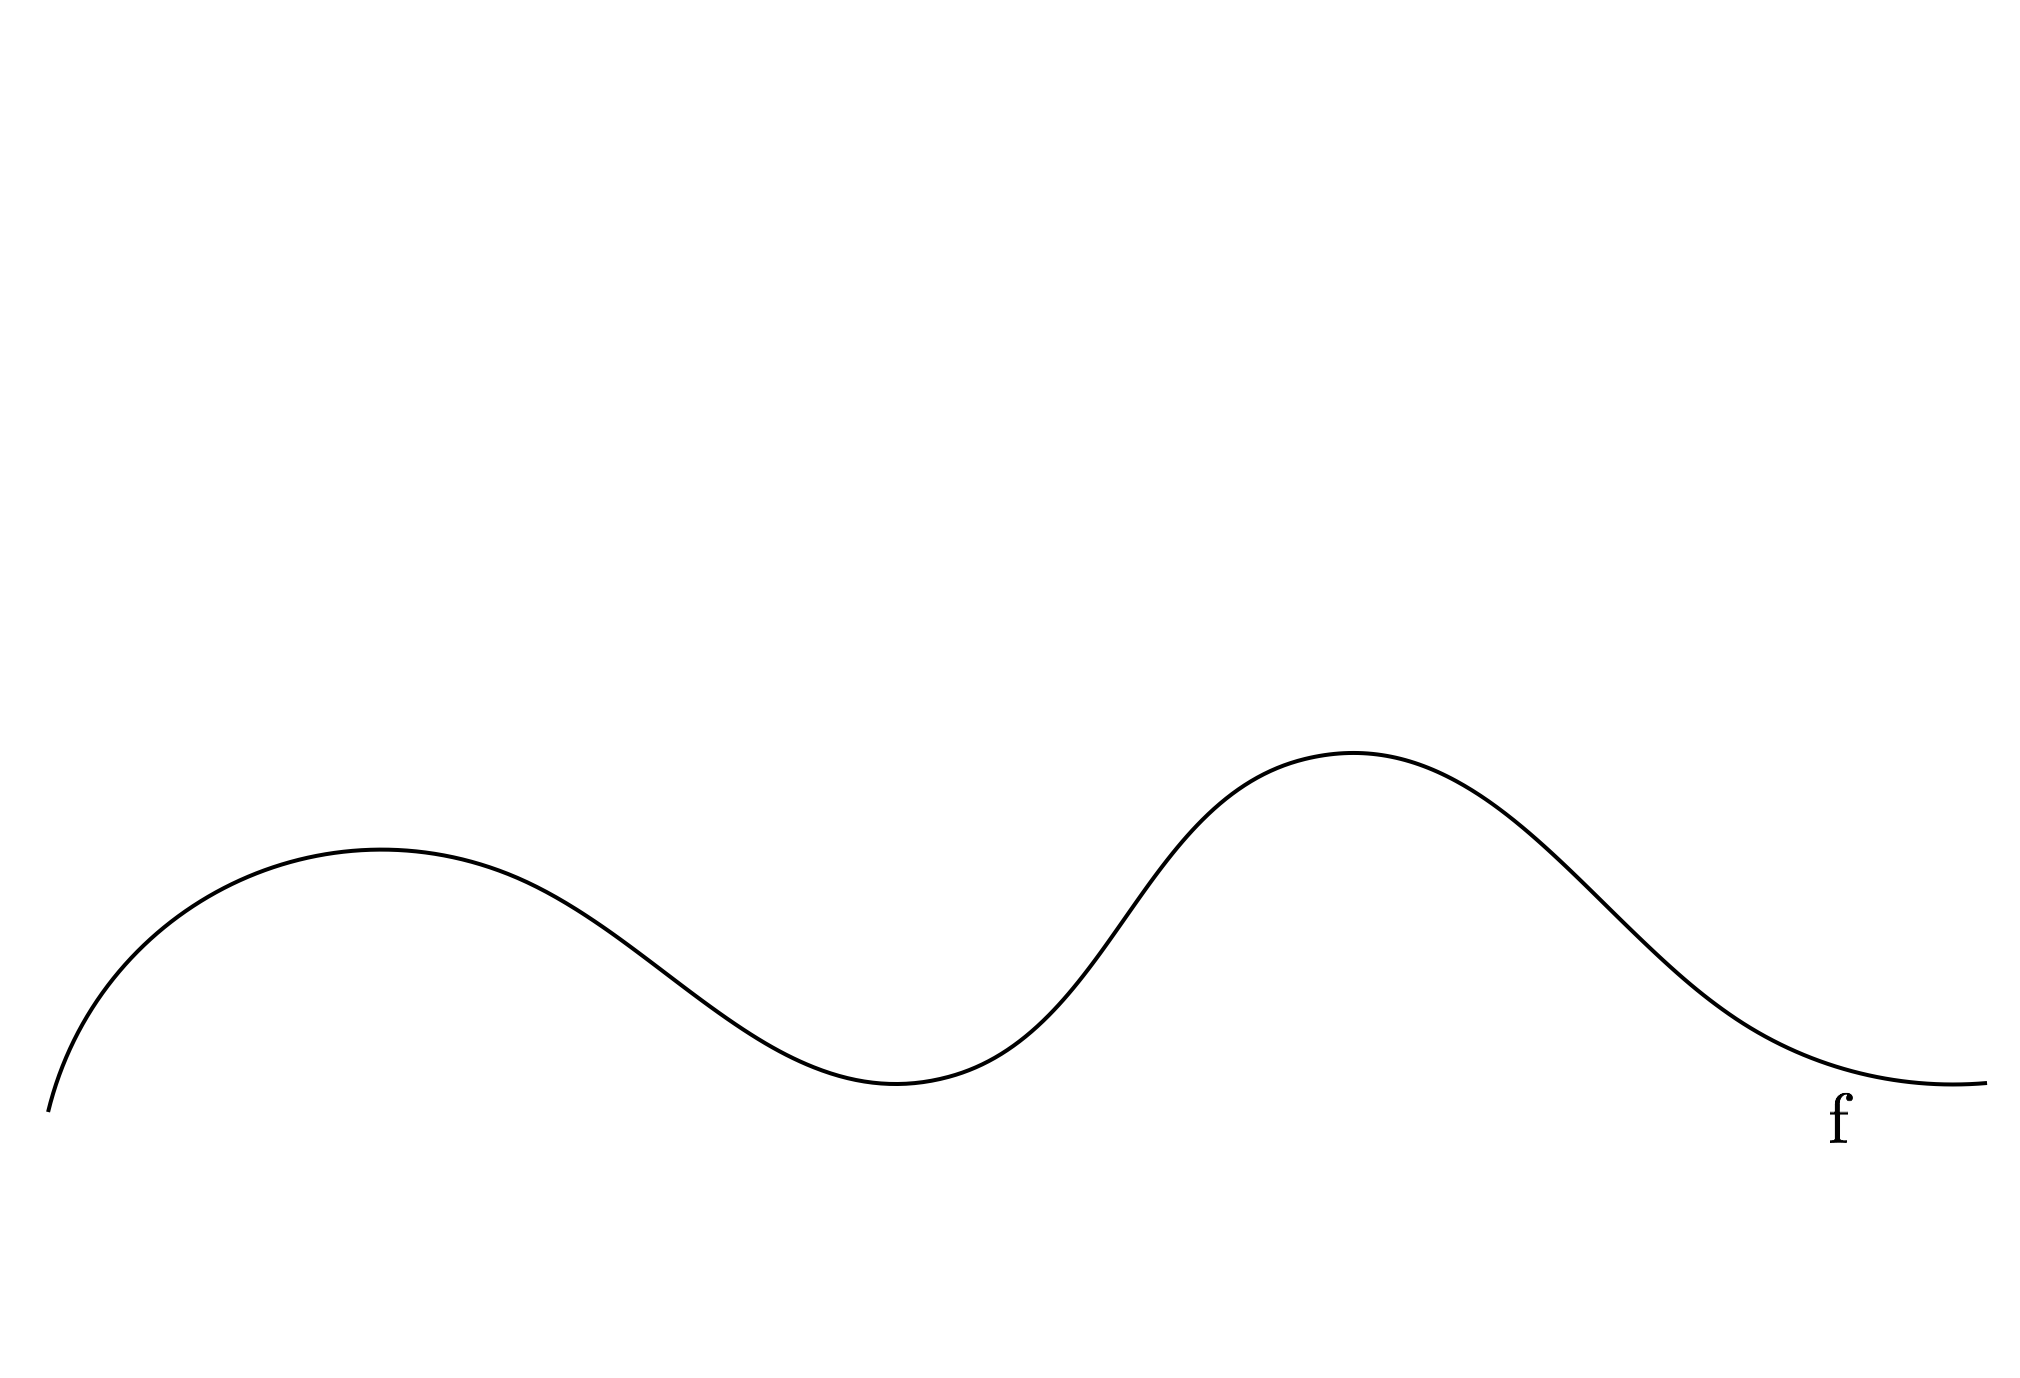
\includegraphics[width=0.8\textwidth]{f}
  \end{center}
  \caption{Visualizing just f.}
\end{figure}



}

\frame{


\begin{figure}
  \begin{center}
    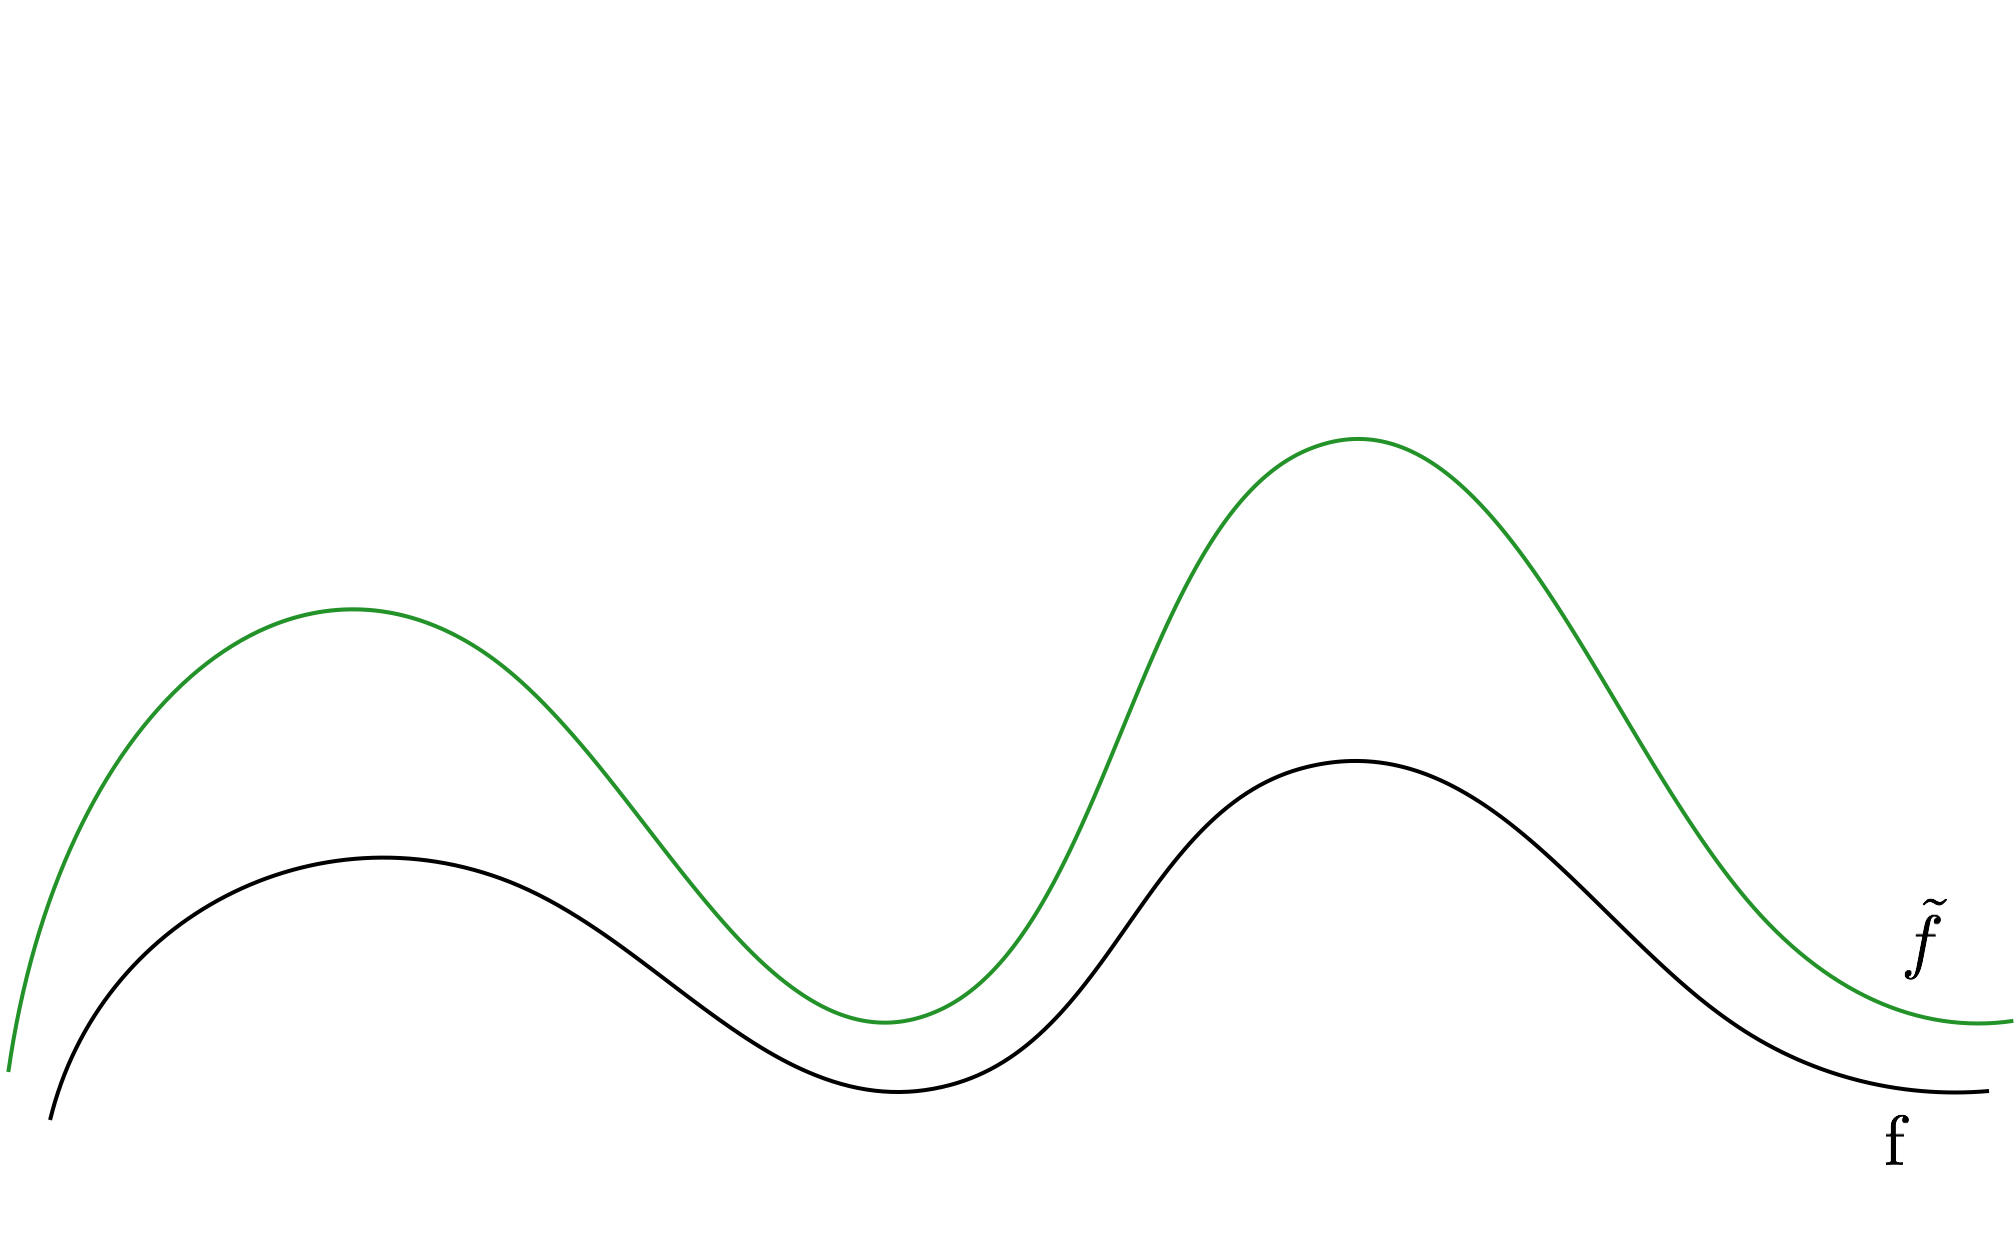
\includegraphics[width=0.8\textwidth]{bothf}
  \end{center}
  \caption{Visualizing just f and $\tilde{f}.$}
\end{figure}



}

\frame{


\begin{figure}
  \begin{center}
    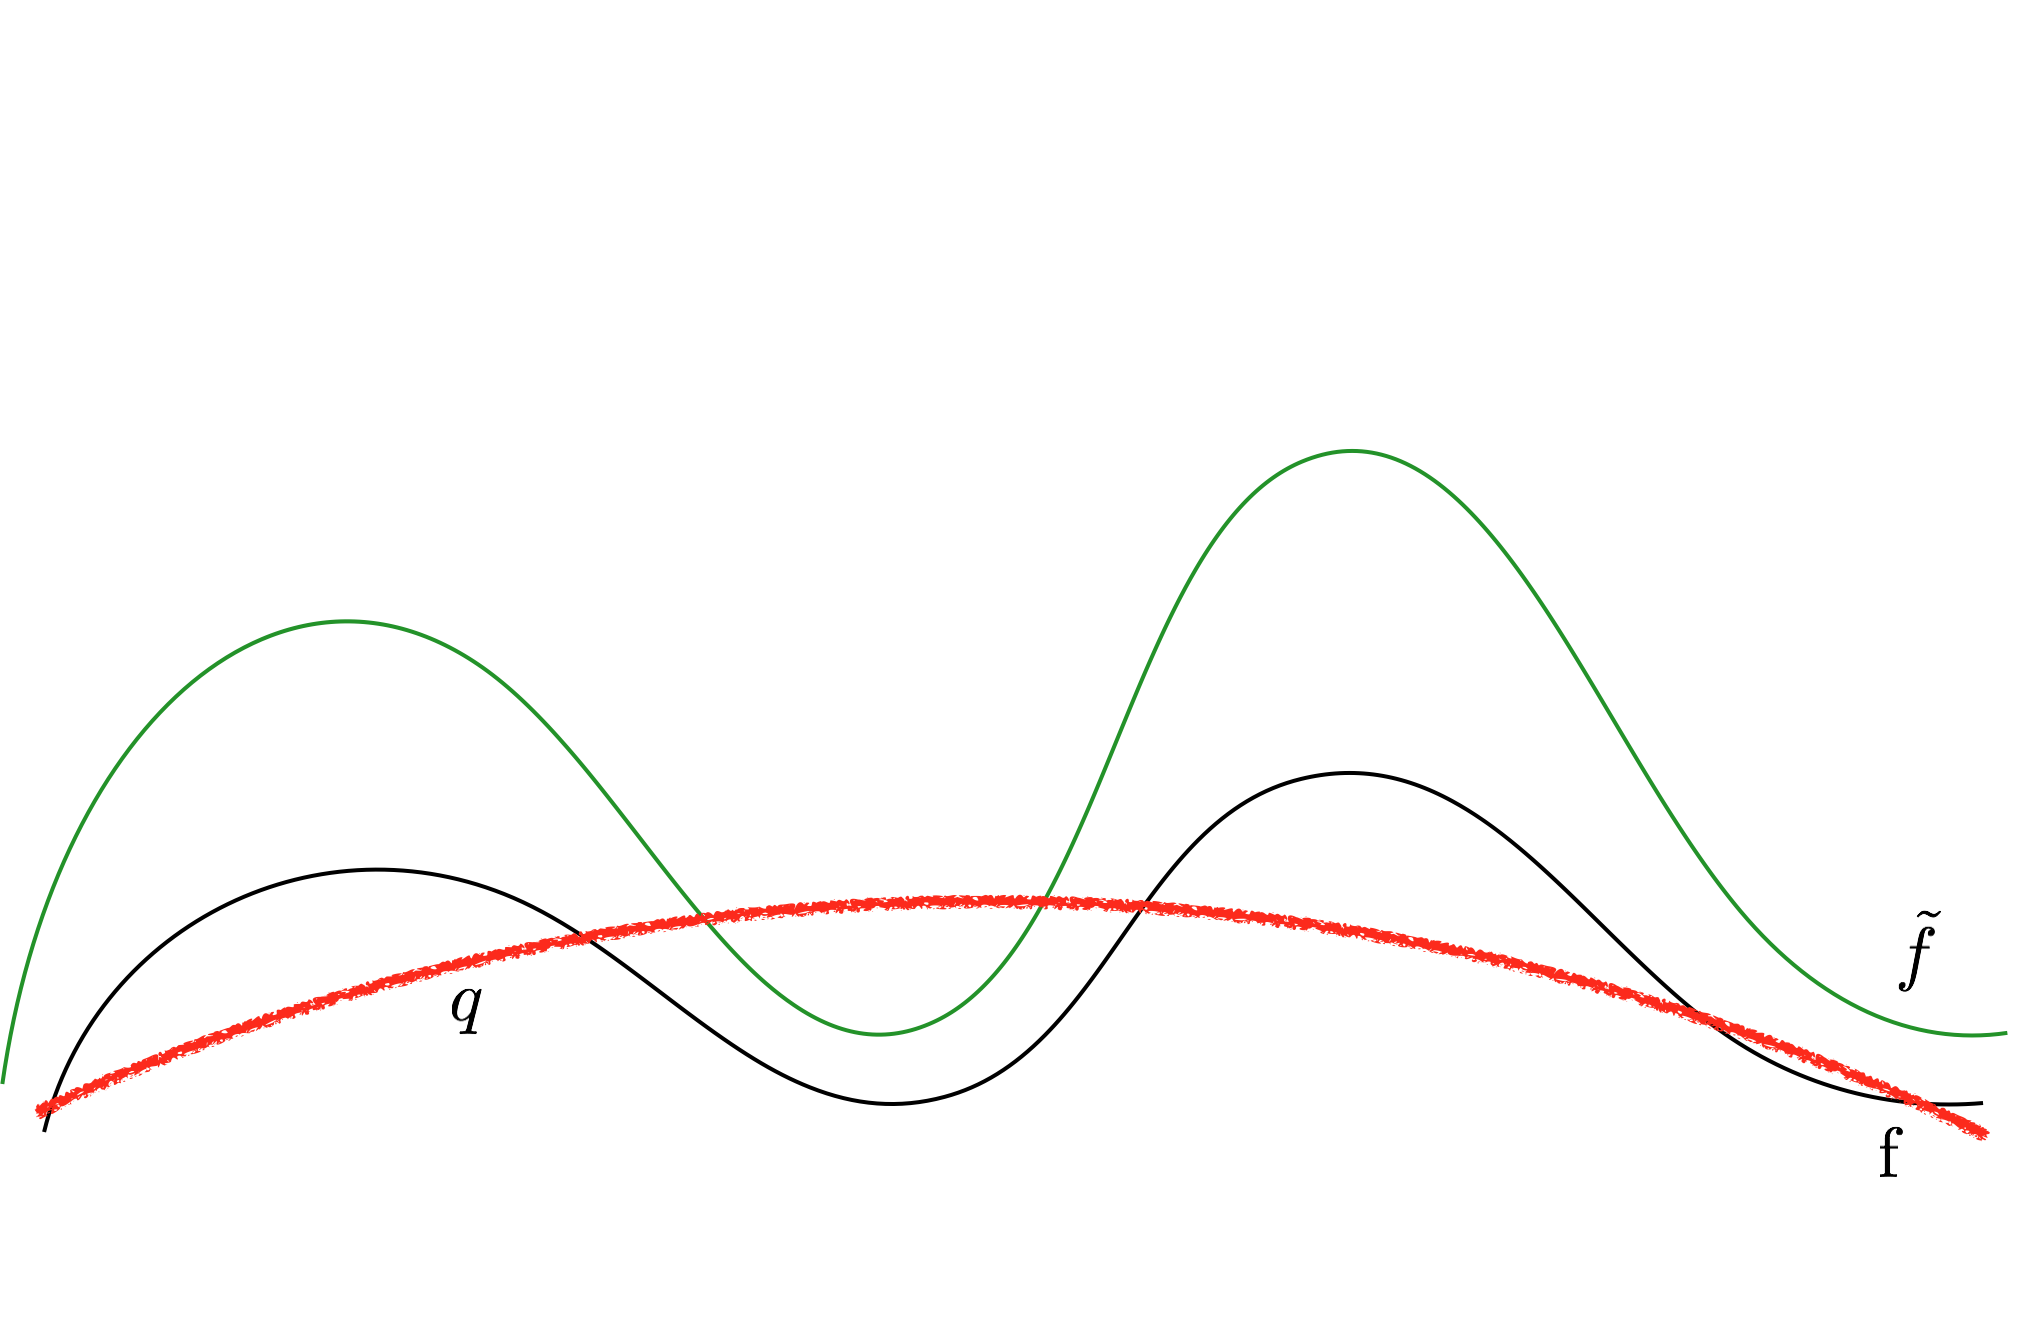
\includegraphics[width=0.8\textwidth]{q}
  \end{center}
  \caption{Visualizing f and $\tilde{f}.$ Now we look at enveloping $q$ over $f.$}
\end{figure}



}

\frame{


\begin{figure}
  \begin{center}
    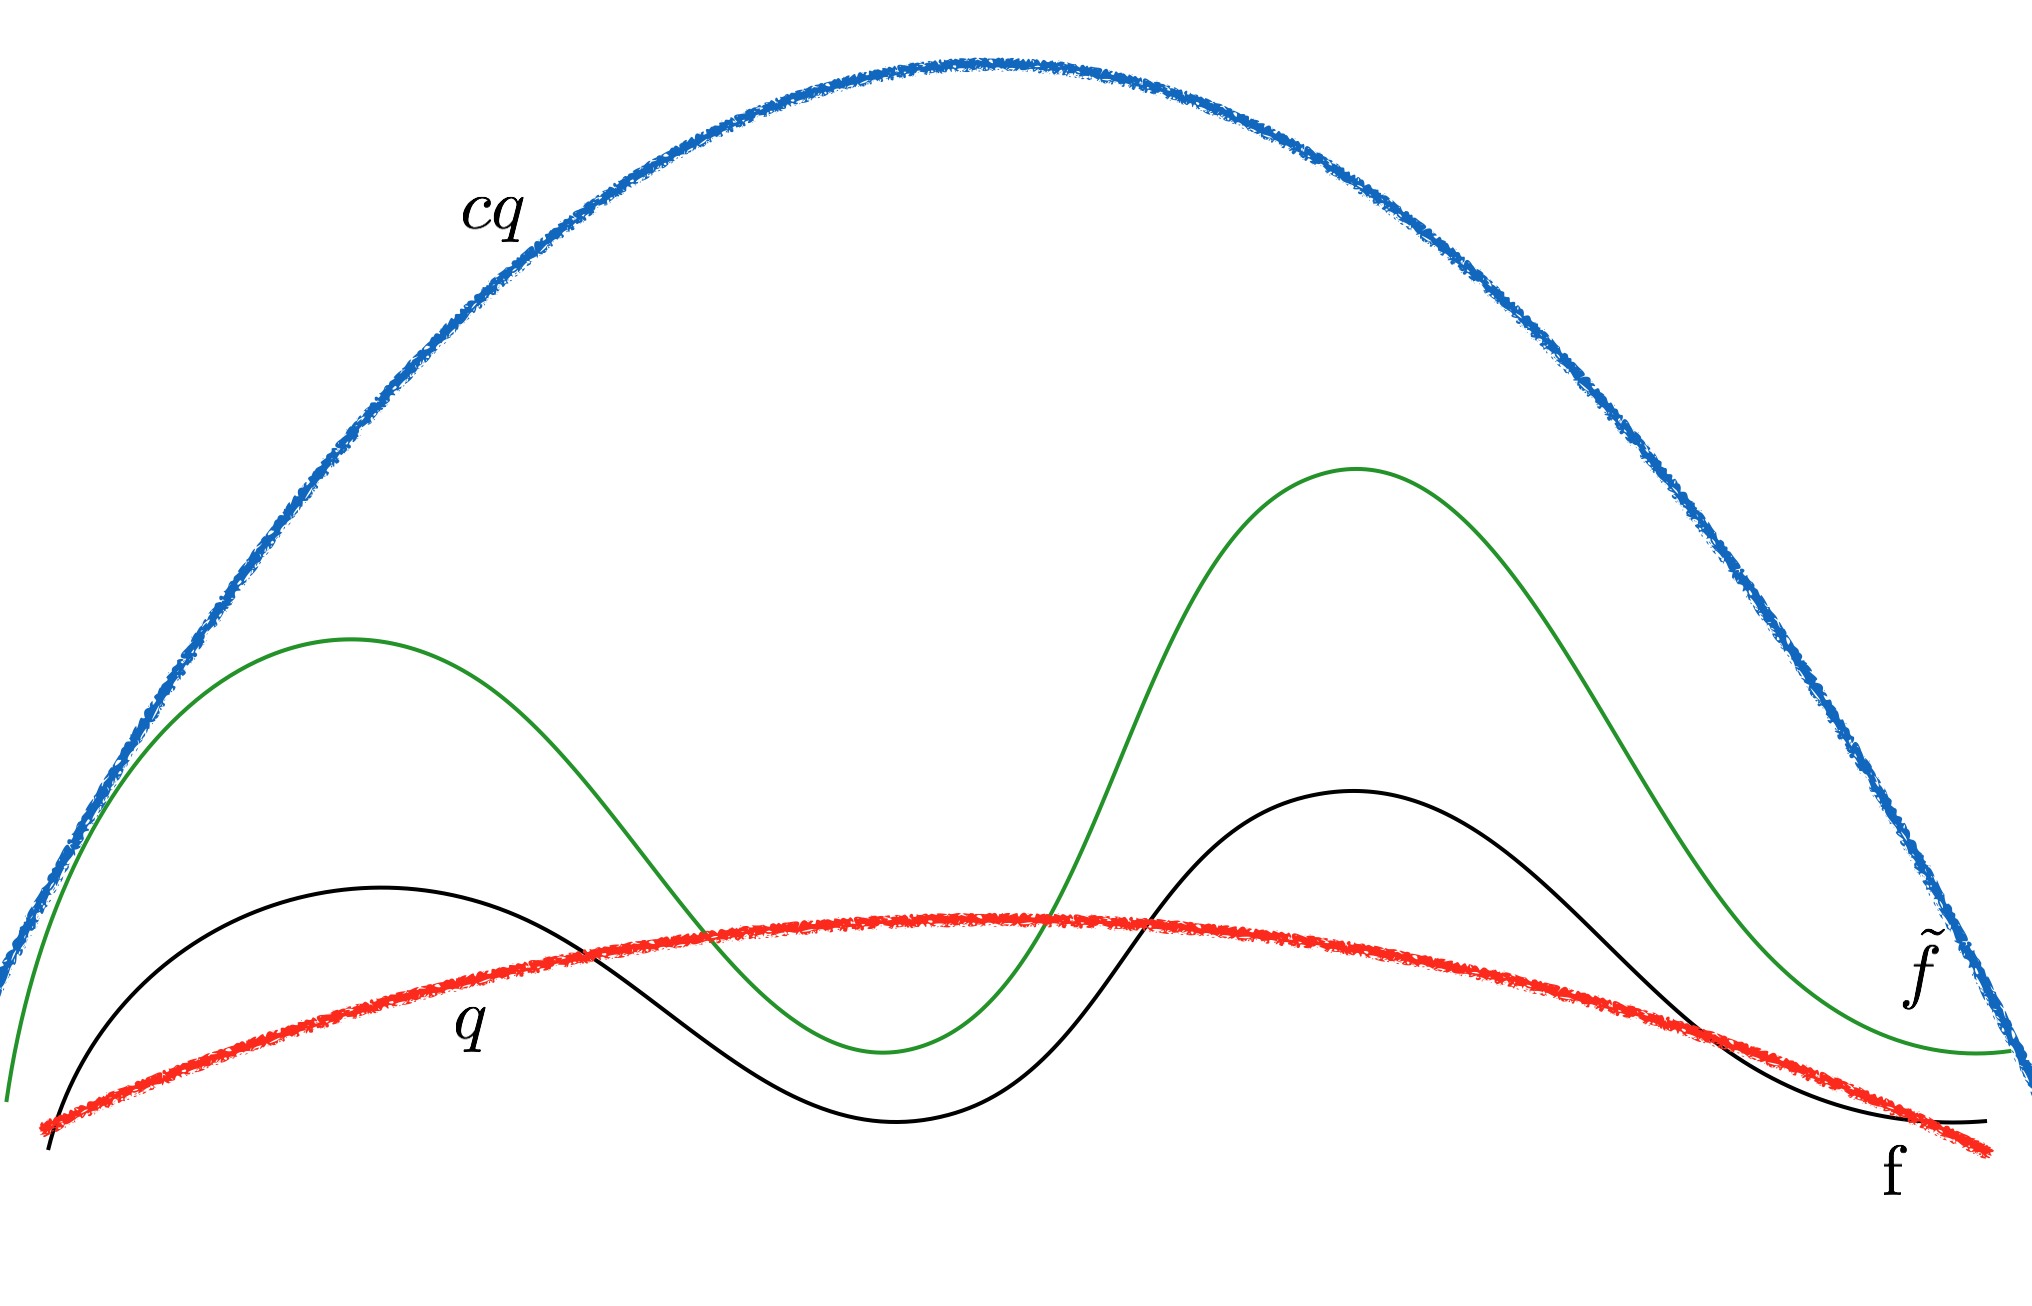
\includegraphics[width=0.8\textwidth]{cq}
  \end{center}
  \caption{Visualizing f and $\tilde{f}.$ Now we look at enveloping $cq$ over $\tilde{f}.$}
\end{figure}



}

\frame{


\begin{figure}
  \begin{center}
    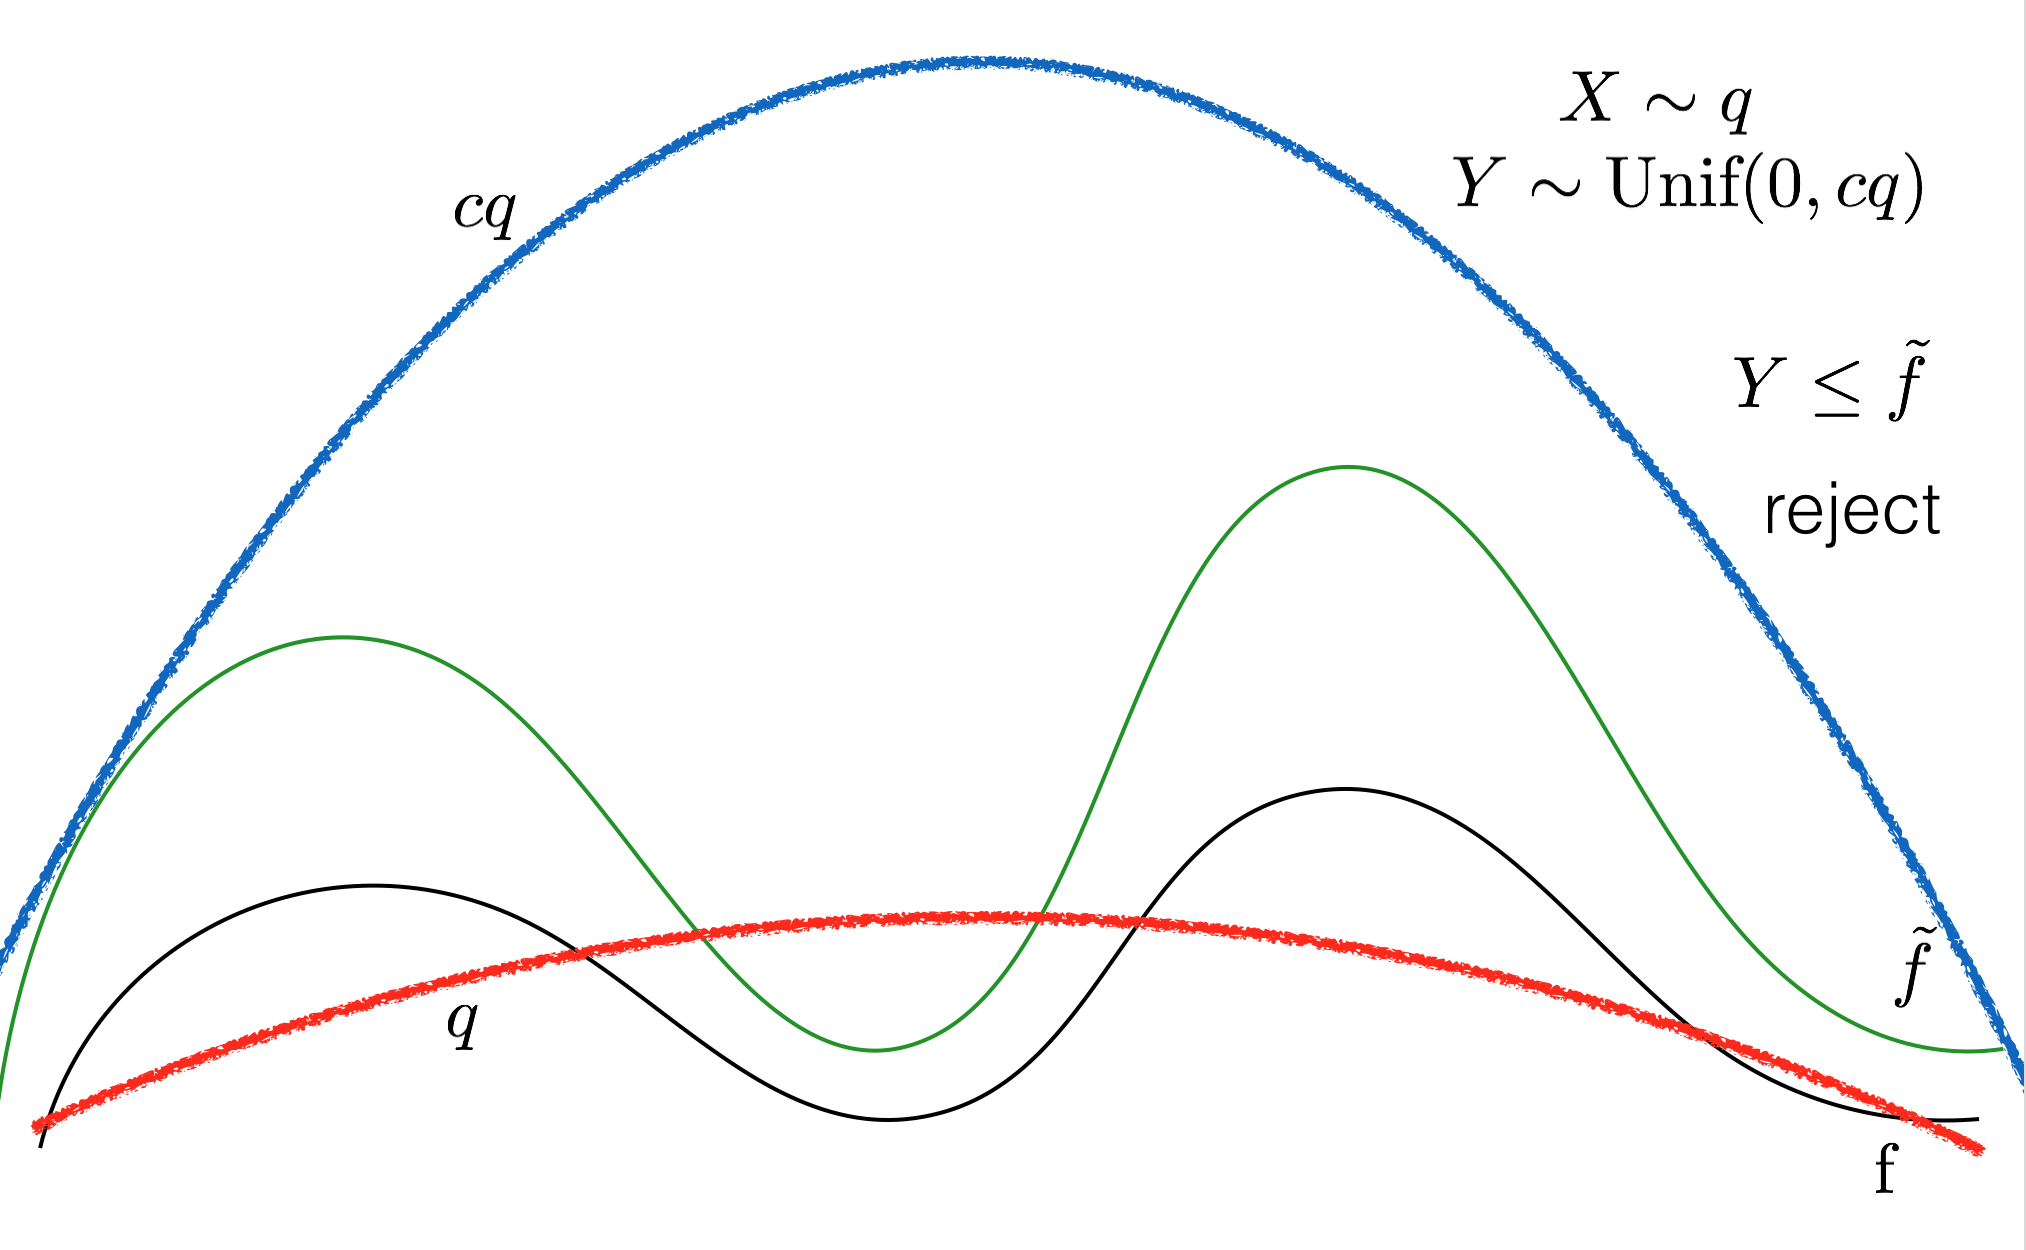
\includegraphics[width=0.8\textwidth]{rejection}
  \end{center}
  \caption{Recalling the sampling method and accept/reject step.}
\end{figure}



}

\frame{


\begin{figure}
  \begin{center}
    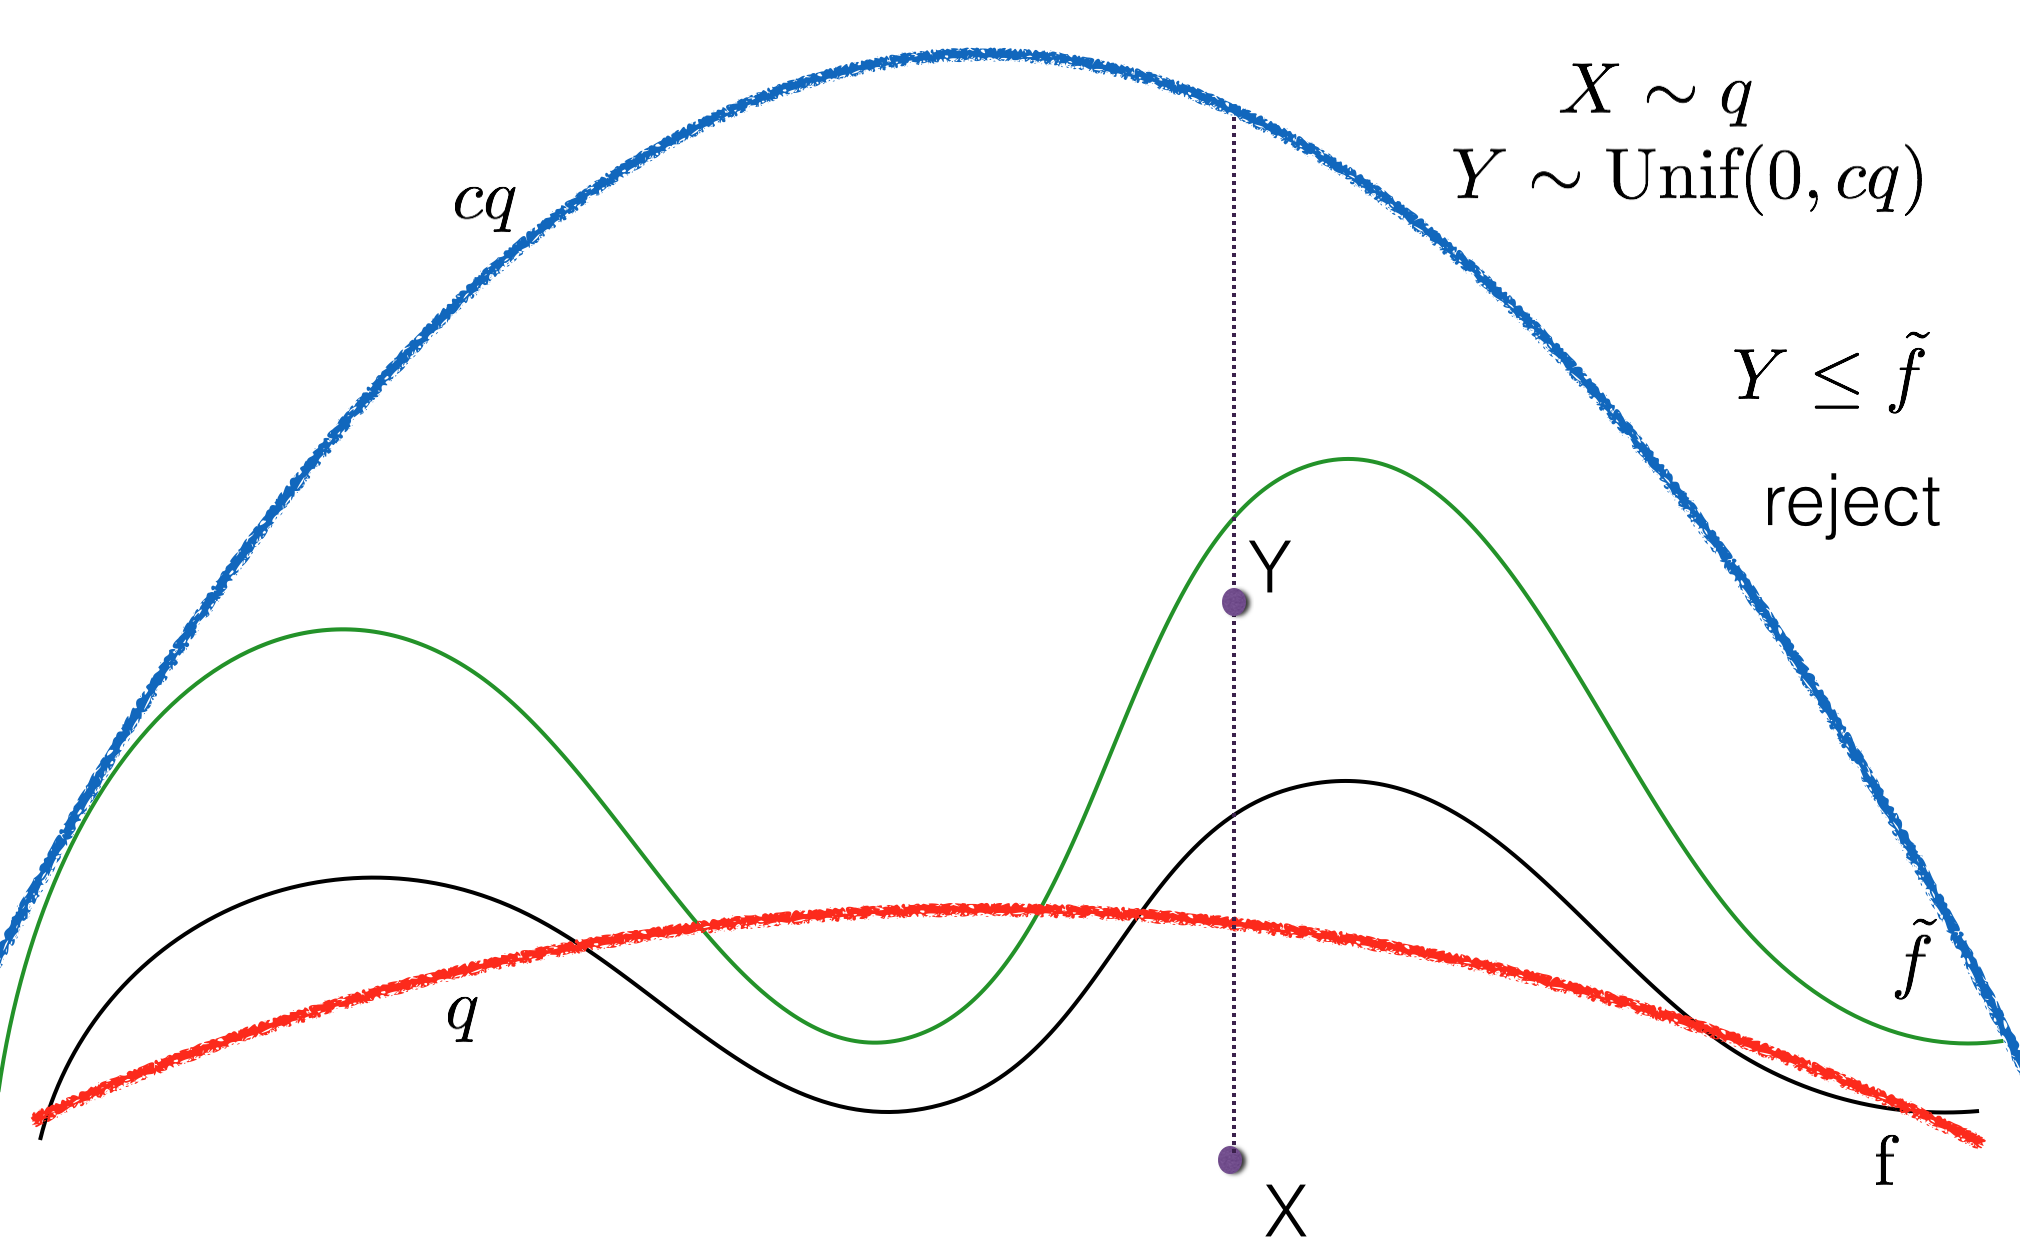
\includegraphics[width=0.8\textwidth]{rejectionEx}
  \end{center}
  \caption{Entire picture and an example point $X$ and $Y.$}
\end{figure}




}

\frame{

\begin{itemize}
\item Suppose we want to generate random variables from the Beta(5.5,5.5) distribution. 
\item There are no direct methods for generating from Beta(a,b) if a,b are not integers. 
\item One possibility is to use a Uniform(0,1) as the trial distribution. A better idea is to use an approximating normal distribution. 
\item Do this as an exercise on your own.
\end{itemize}
}


%%%start here
%\begin{frame}[fragile]
%\begin{verbatim}
%##simple rejection sampler for Beta(5.5,5.5)
%a <- 5.5; b <- 5.5
%m <- a/(a+b); s <- sqrt((a/(a+b))*(b/(a+b))/(a+b+1))
%funct1 <- function(x) {dnorm(x, mean=m, sd=s)}
%funct2 <- function(x) {dbeta(x, shape1=a, shape2=b)}
%
%##plotting normal and beta densities
%plot(funct1, from=0, to=1, col="blue", ylab="")
%plot(funct2, from=0, to=1, col="red", add=T)
%
%
%##M=1.3 (this is trial and error to get a good M)
%funct1 <- function(x) {1.3*dnorm(x, mean=m, sd=s)}
%funct2 <- function(x) {dbeta(x, shape1=a, shape2=b)}
%plot(funct1, from=0, to=1, col="blue", ylab="")
%plot(funct2, from=0, to=1, col="red", add=T)
%\end{verbatim}
%\end{frame}
%
%%%start here
%\begin{frame}[fragile]
%\begin{verbatim}
%
%##Doing accept-reject
%##substance of code
%set.seed(1); nsim <- 1e5
%x <- rnorm(n=nsim, mean=m, sd=s)
%u <- runif(n=nsim)
%ratio <- dbeta(x, shape1=a, shape2=b) /
%           (1.3*dnorm(x, mean=m, sd=s))
%ind <- I(u < ratio)
%betas <- x[ind==1]
%# as a check to make sure we have enough
%length(betas) # gives 76836
%
%funct2 <- function(x) {dbeta(x, shape1=a, shape2=b)}
%pdf(file = "beta3.pdf", height = 4.5, width = 5)
%plot(density(betas))
%plot(funct2, from=0, to=1, col="red", lty=2, add=T)
%dev.off()
%\end{verbatim}
%\end{frame}
%
%\frame{
%
%\begin{figure}[htbp]
%\begin{minipage}[b]{0.45\linewidth}
%\centering
%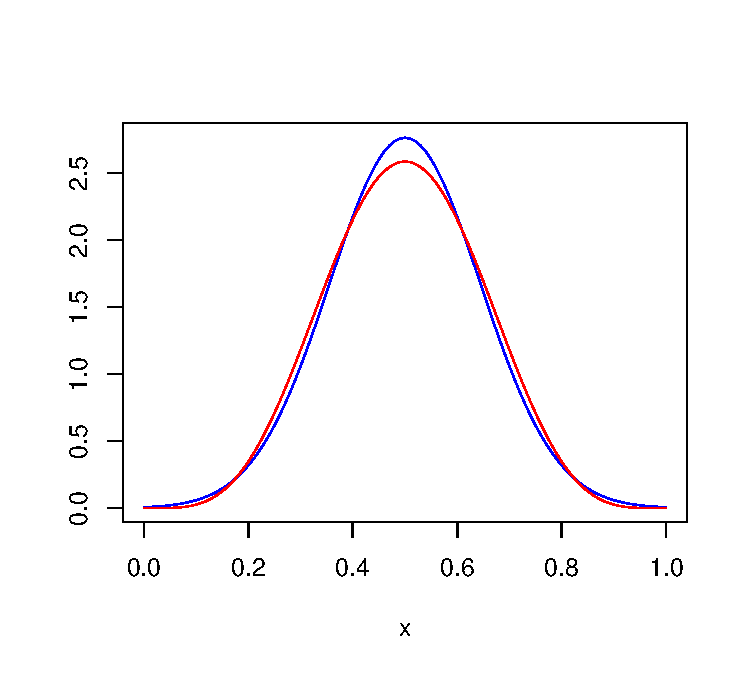
\includegraphics[width=\textwidth]{beta1.pdf}
%\caption{Normal enveloping Beta}
%\label{fig:figure1}
%\end{minipage}
%\hspace{0.5cm}
%\begin{minipage}[b]{0.45\linewidth}
%\centering
%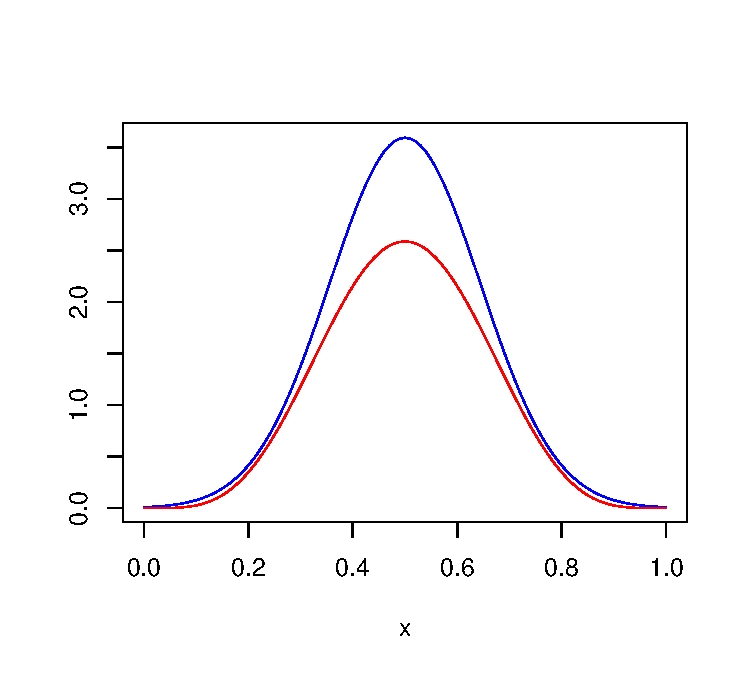
\includegraphics[width=\textwidth]{beta2.pdf}
%\caption{Naive rejection sampling, M=1.3}
%\label{fig:figure2}
%\end{minipage}
%\end{figure}
%
%
%}
%
%
%\frame{
%
%\begin{figure}[htbp]
%\begin{center}
%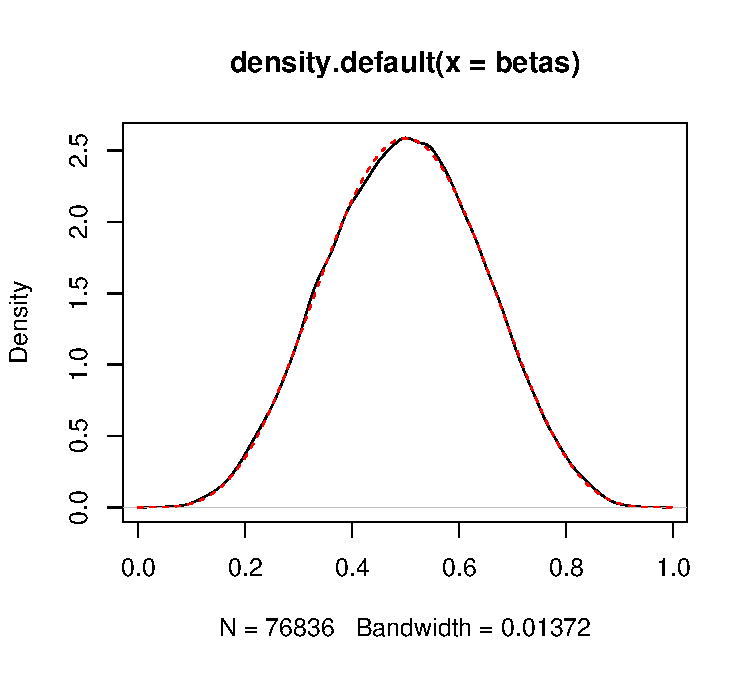
\includegraphics[width=0.5\textwidth]{beta3.pdf}
%\caption{Rejection sampler}
%\label{default}
%\end{center}
%\end{figure}
%
%
%
%}

\end{document}